\chapter{Resultados} 
\label{cap5_resultados}

\section{Front-end}

\subsection{Protótipos}

Após a reunião de levantamento de requisitos, protótipos das telas principais da plataforma foram construídos no Figma para validação junto ao setor. Esses protótipos estão disponíveis no repositório do projeto, no endereço \url{https://github.com/Tomaz5556/Horarios-IFNMG-Salinas/blob/main/prototipos/figma.pdf}. A seguir, são apresentadas as telas desenvolvidas:

\begin{figure}[htb]
    \centering
    \caption{Protótipo da tela inicial}
    
\includegraphics[width=1\textwidth]{Figuras/proto-1.png}
    \caption*{Fonte: AUTOR (2024)}
    \label{fig_proto_1}
\end{figure}

A Figura \ref{fig_proto_1} exibe o protótipo da tela inicial da plataforma, onde o usuário encontra quatro opções para selecionar o tipo de horário.

\begin{figure}[H]
    \centering
    \caption{Protótipo da tela dos cursos}
    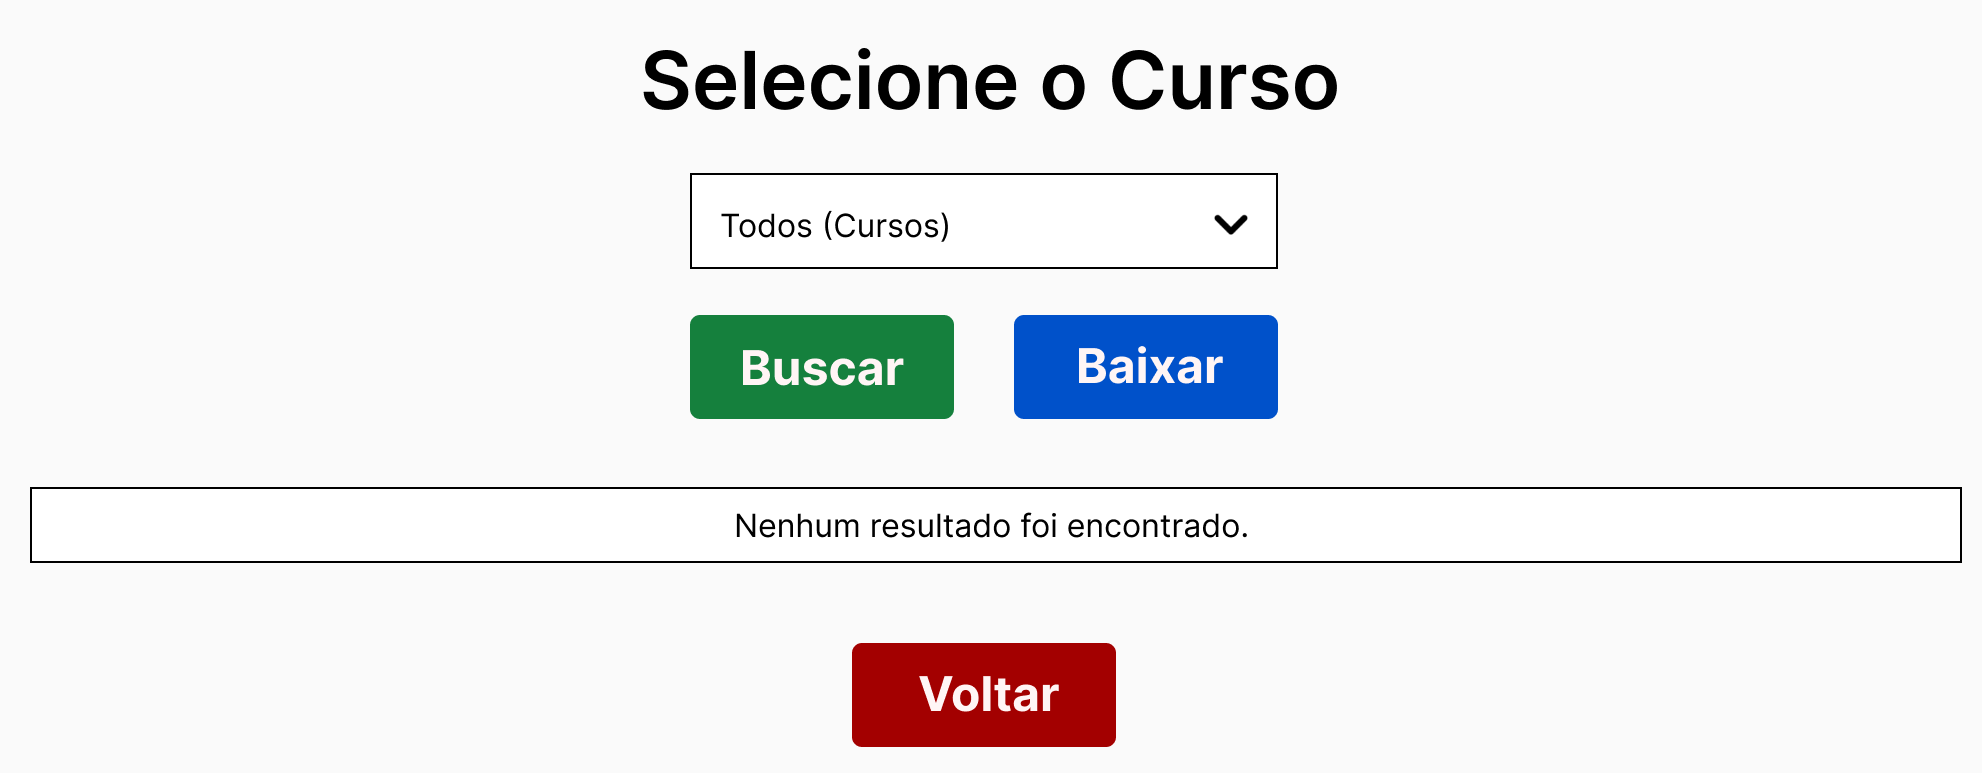
\includegraphics[width=1\textwidth]{Figuras/proto-2.PNG}
    \caption*{Fonte: AUTOR (2024)}
    \label{fig_proto_2}
\end{figure}

\begin{figure}[htb]
    \centering
    \caption{Protótipo da tela dos cursos preenchida}
    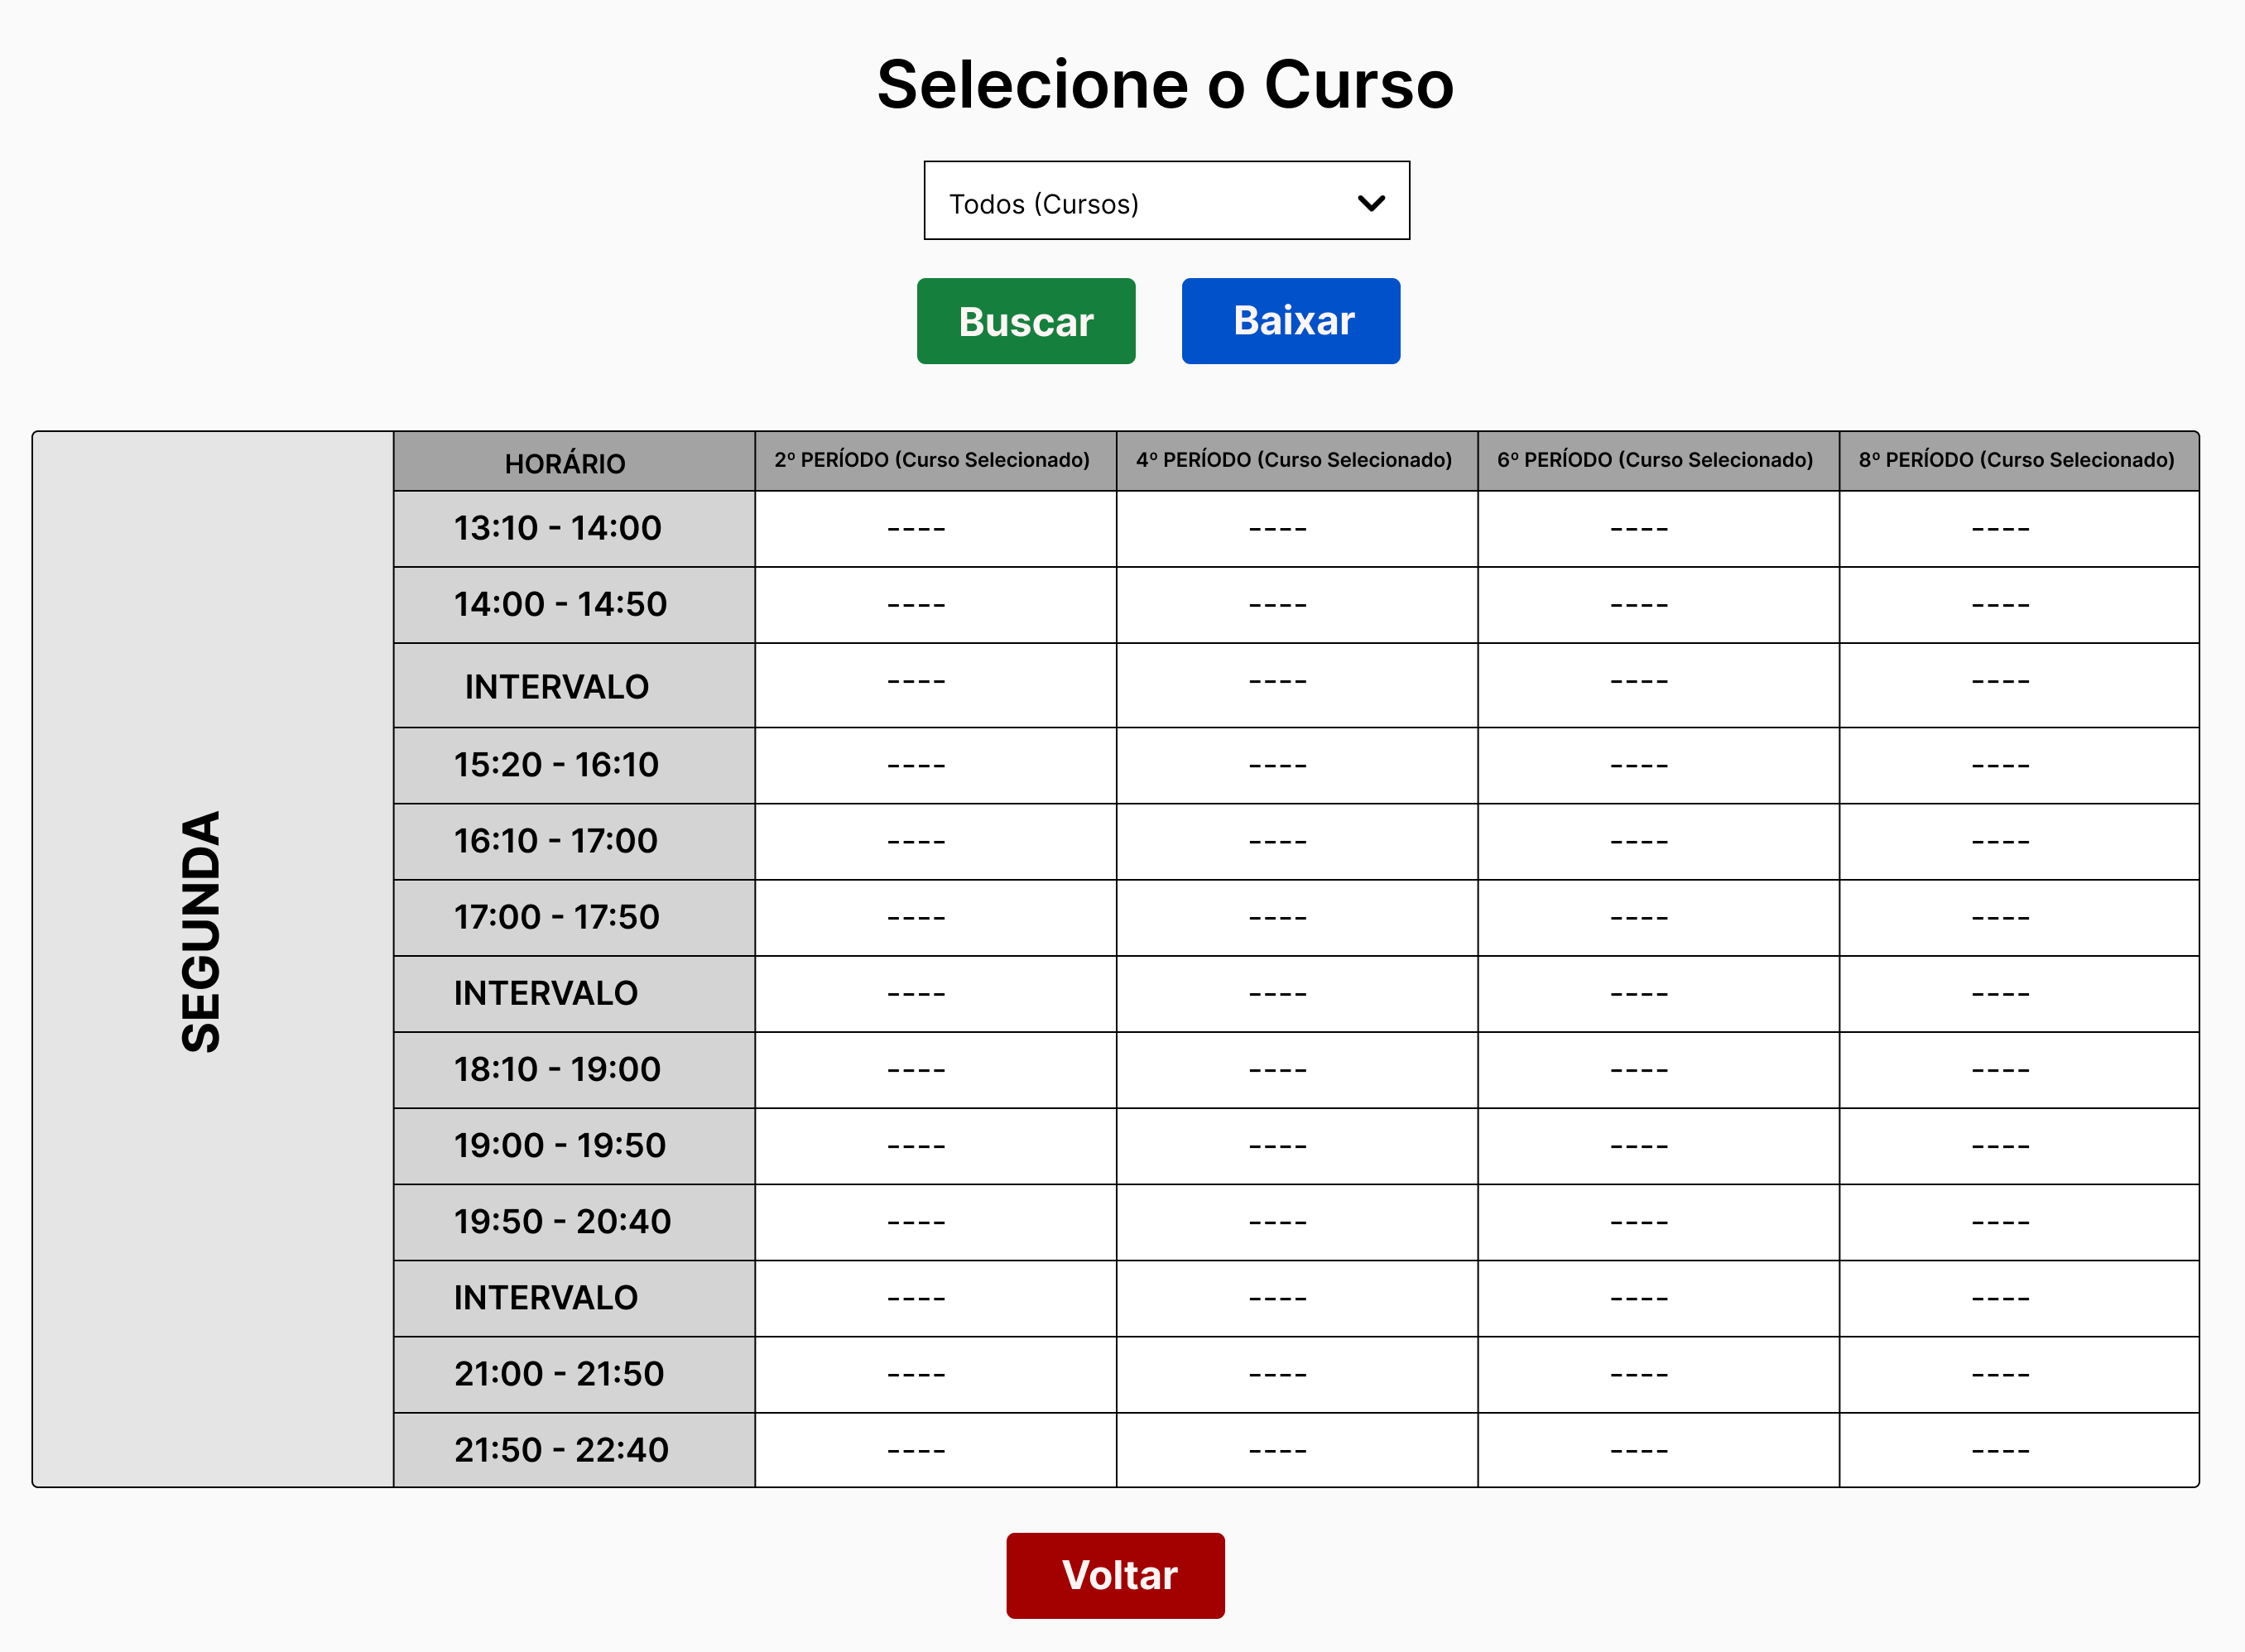
\includegraphics[width=1\textwidth]{Figuras/proto-3.PNG}
    \caption*{Fonte: AUTOR (2024)}
    \label{fig_proto_3}
\end{figure}

As Figuras \ref{fig_proto_2} e \ref{fig_proto_3} apresentam o protótipo da tela dos cursos, exibindo os horários e a distribuição das aulas ao longo da semana para um curso selecionado.

\begin{figure}[htb]
    \centering
    \caption{Protótipo da tela dos professores}
    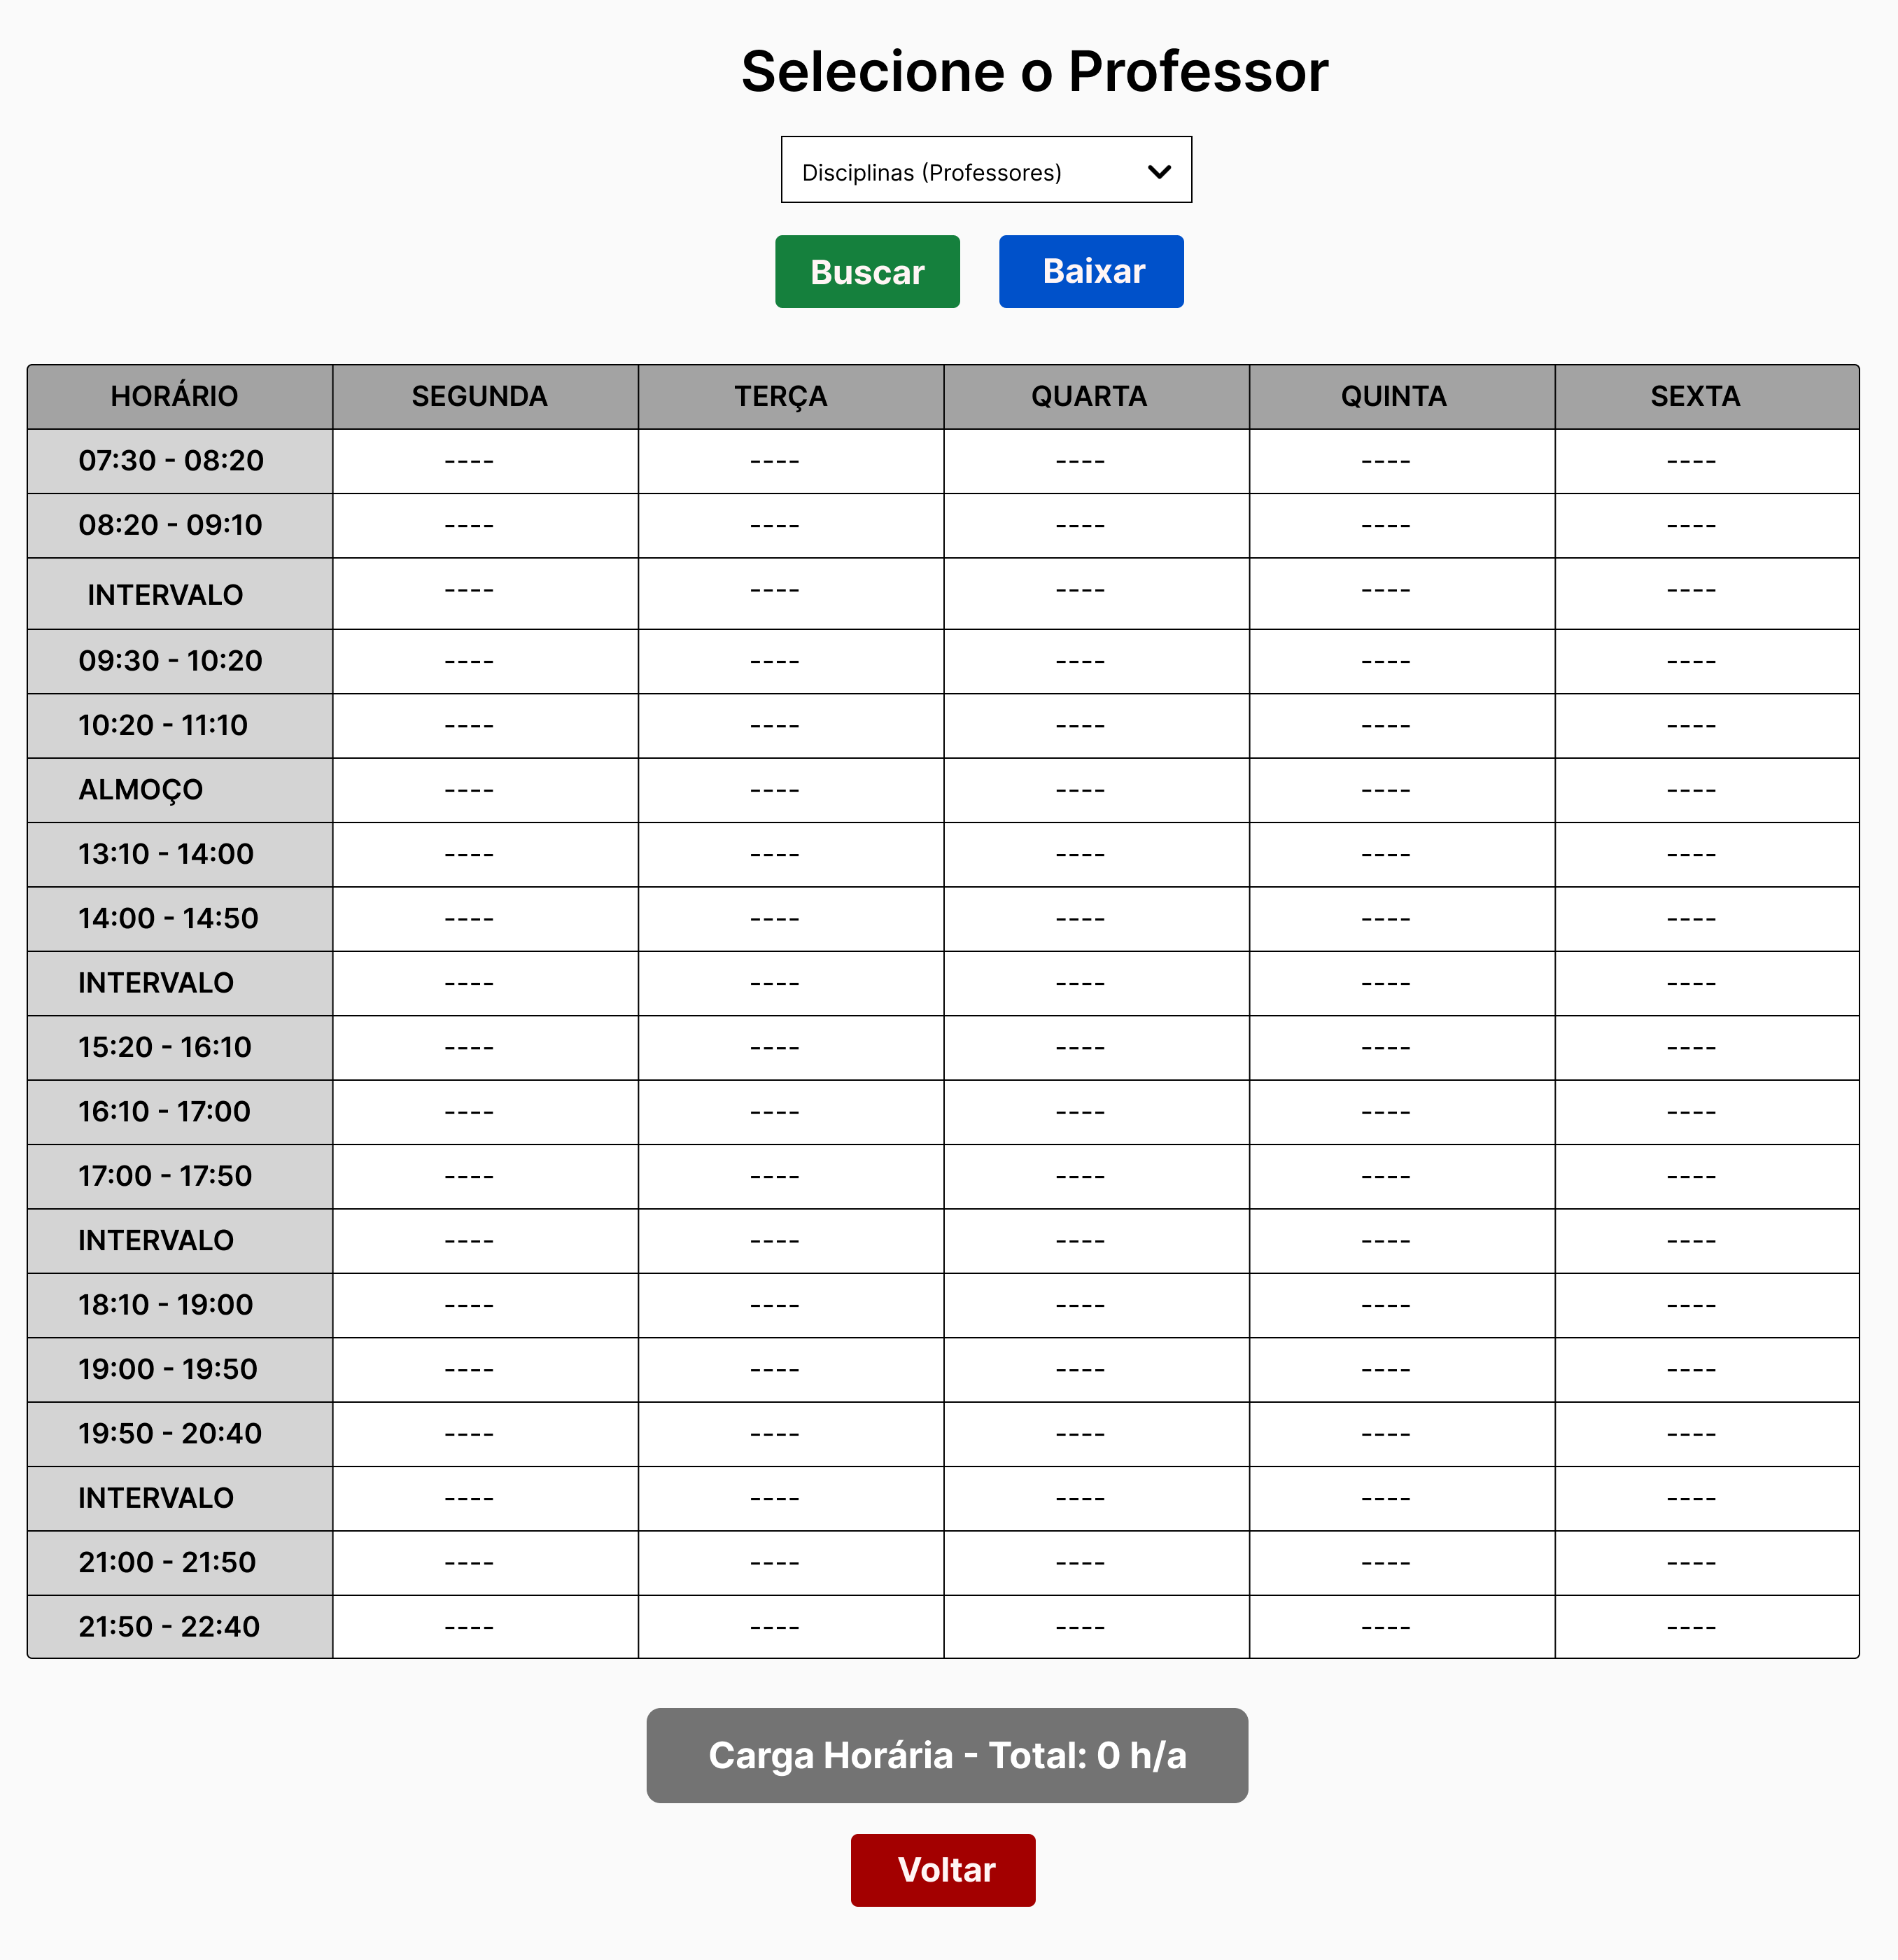
\includegraphics[width=1\textwidth]{Figuras/proto-4.PNG}
    \caption*{Fonte: AUTOR (2024)}
    \label{fig_proto_4}
\end{figure}

A Figura \ref{fig_proto_4} mostra o protótipo da tela dos professores, detalhando os horários das aulas e os dias da semana de um professor escolhido.

\begin{figure}[H]
    \centering
    \caption{Protótipo da tela das salas}
    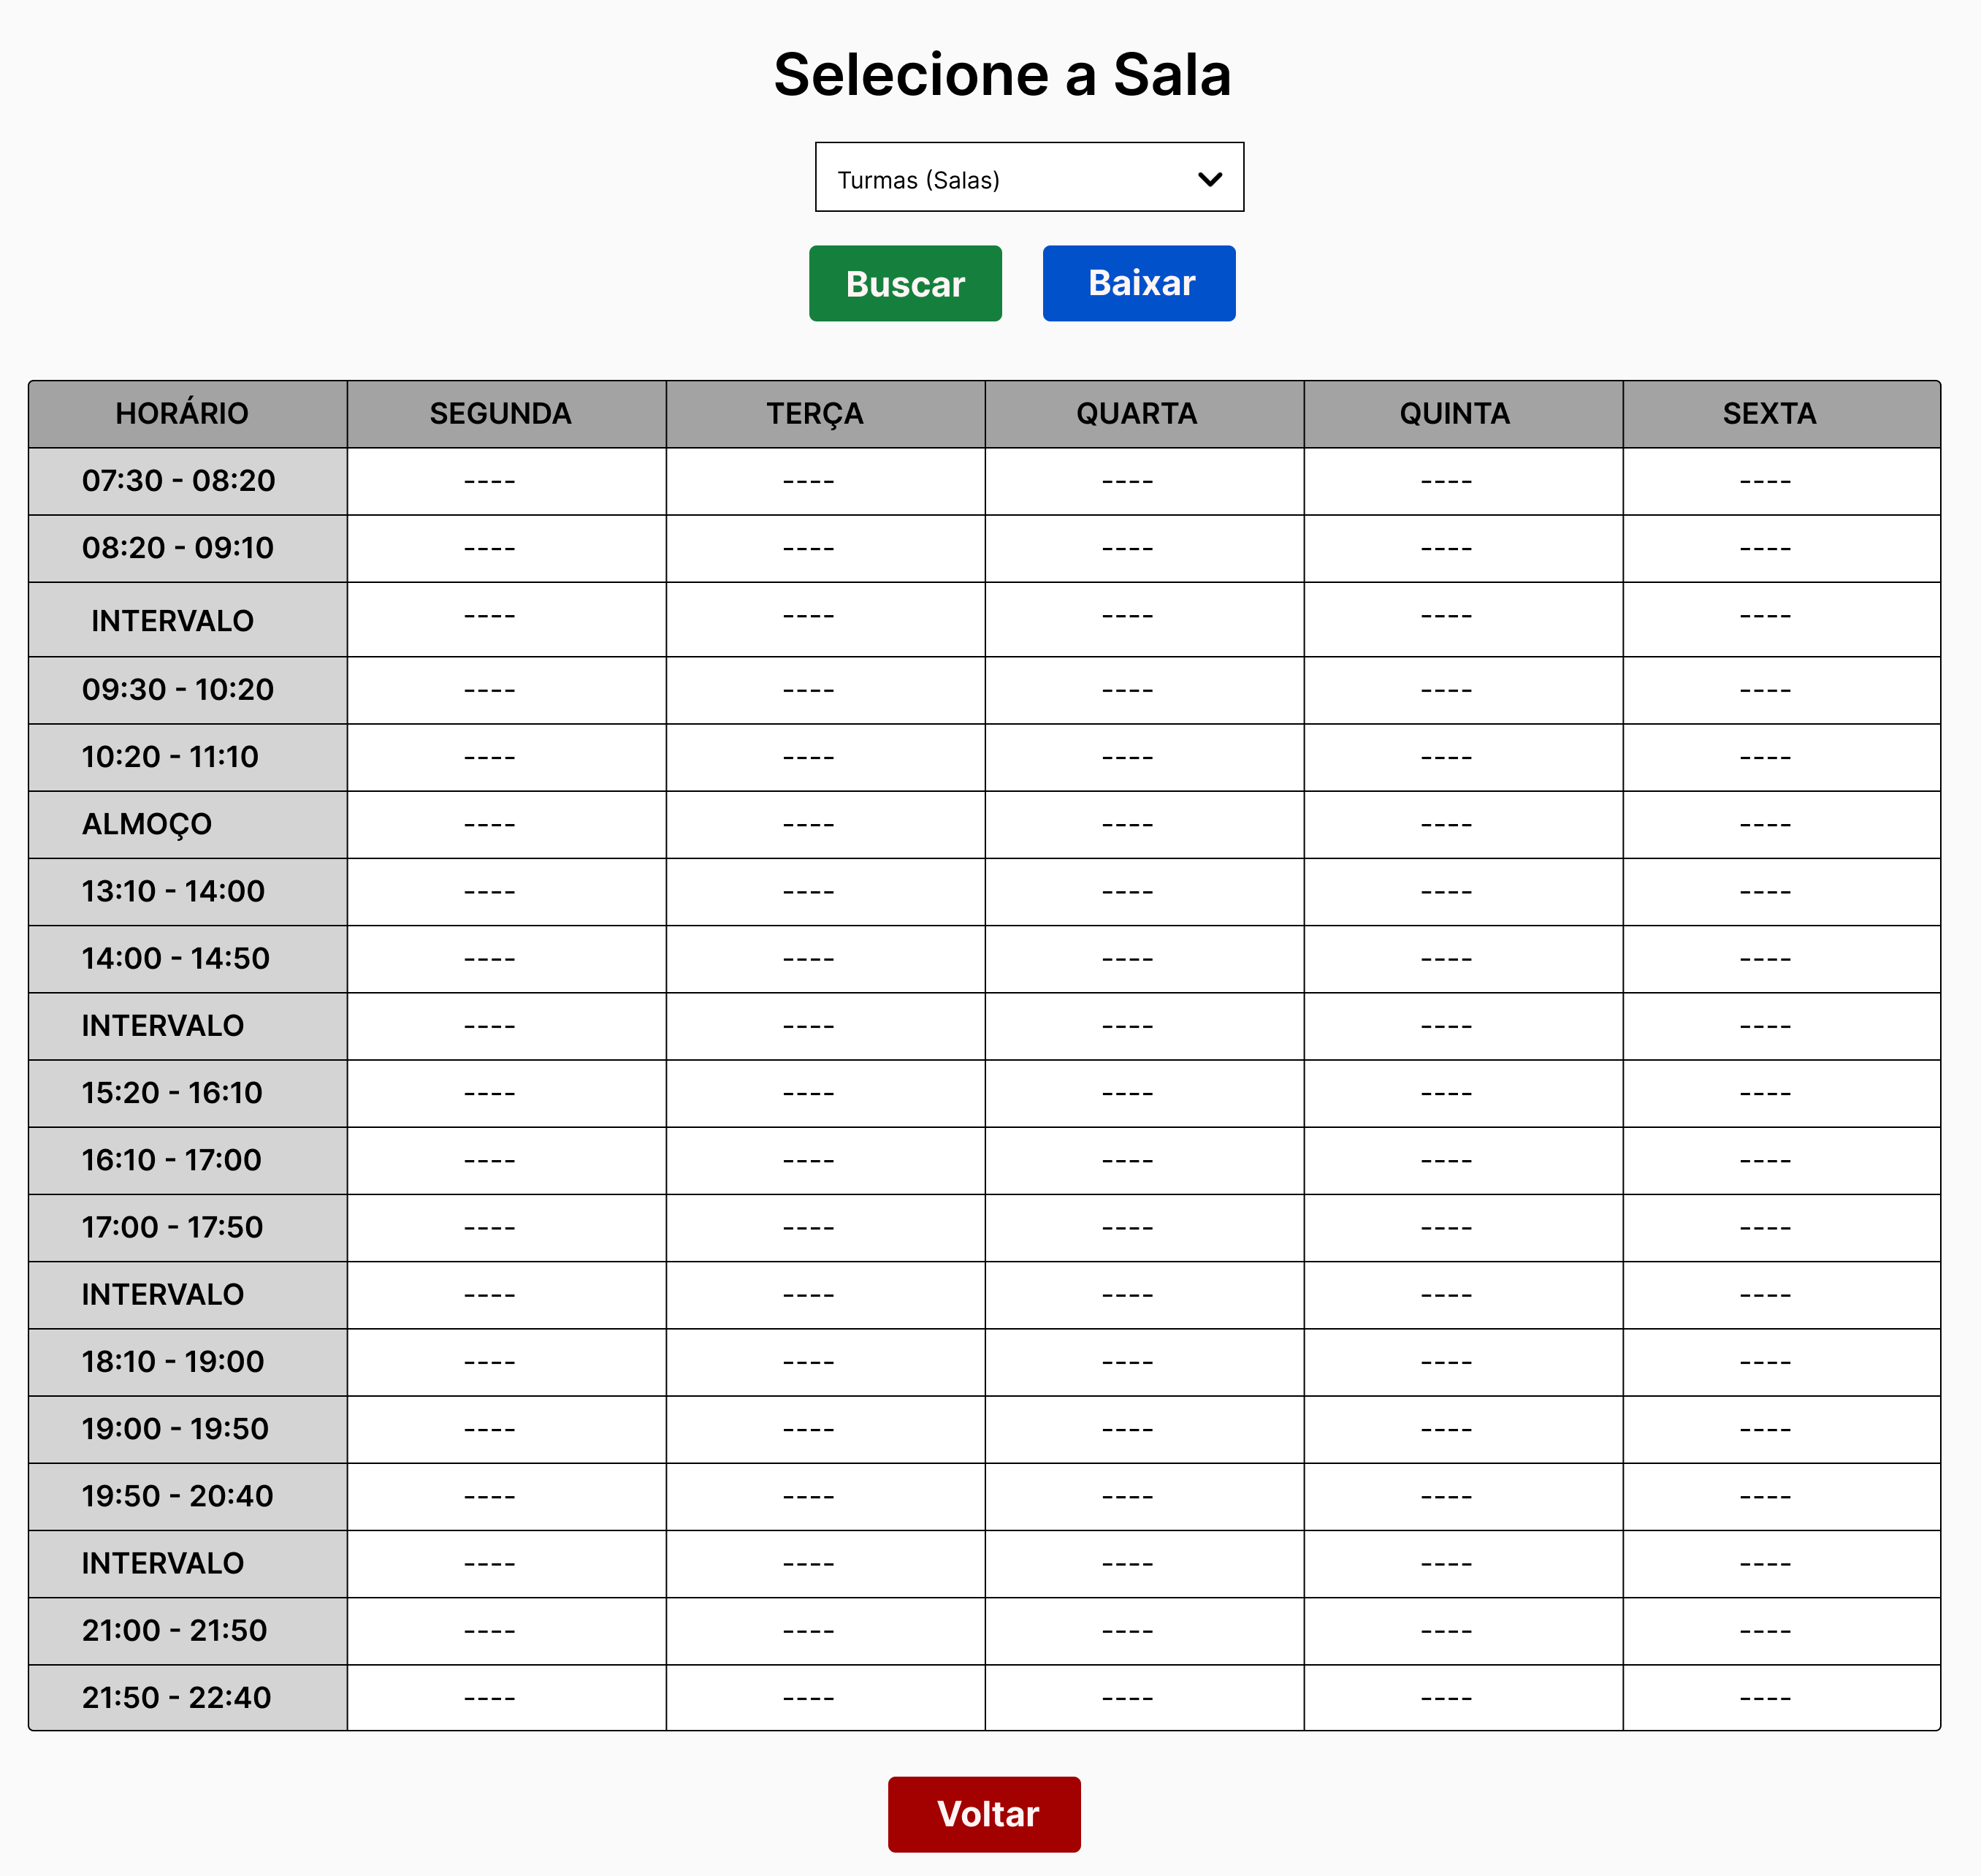
\includegraphics[width=1\textwidth]{Figuras/proto-5.PNG}
    \caption*{Fonte: AUTOR (2024)}
    \label{fig_proto_5}
\end{figure}

A Figura \ref{fig_proto_5} apresenta o protótipo da tela das salas, exibindo os horários de ocupação e os dias em que uma sala está reservada.

\subsection{Desenvolvimento do Front-end}

O front-end foi desenvolvido com o Next.js. Essa tecnologia possibilitou criar uma interface moderna e eficiente, capaz de responder dinamicamente a eventos e mudanças de estado, garantindo uma experiência de usuário fluida e responsiva. Todo o trabalho priorizou clareza na organização dos componentes, reutilização de elementos e facilidade de futuras evoluções, atendendo às necessidades do projeto com agilidade. O código está disponível no repositório do projeto em \url{https://github.com/Tomaz5556/Horarios-IFNMG-Salinas/tree/main/frontend}. A seguir, são exibidas as telas resultantes desse processo:

\begin{figure}[htb]
    \centering
    \caption{Menu principal com opções de botões de horários e outros serviços}
    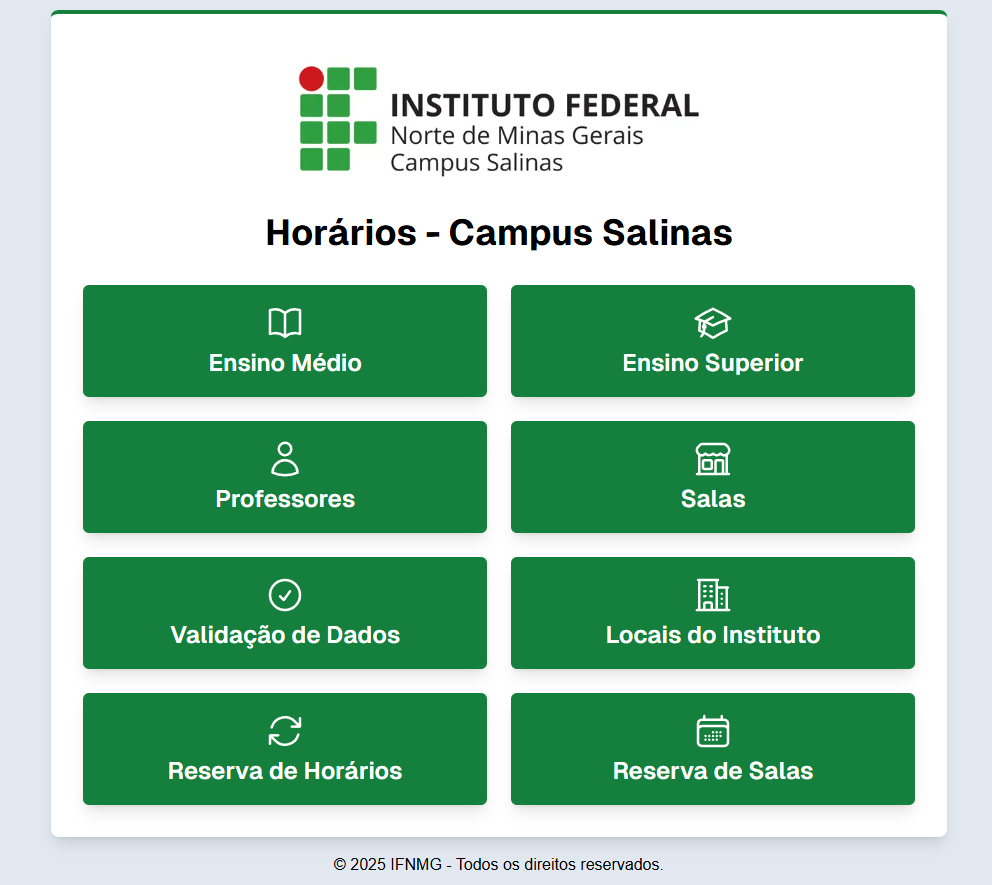
\includegraphics[width=1\textwidth]{Figuras/front-1.png}
    \caption*{Fonte: AUTOR (2025)}
    \label{fig_front_1}
\end{figure}

A Figura \ref{fig_front_1} mostra o menu principal da plataforma, com botões para consulta de horários e acesso a outros serviços.

\begin{figure}[htb]
    \centering
    \caption{Tela dos cursos}
    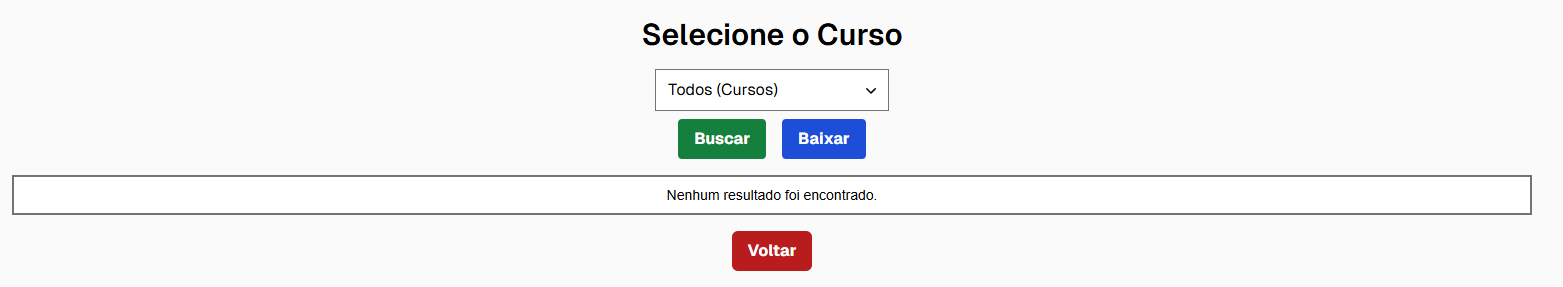
\includegraphics[width=1\textwidth]{Figuras/front-2.png}
    \caption*{Fonte: AUTOR (2025)}
    \label{fig_front_2}
\end{figure}

A Figura \ref{fig_front_2} apresenta a tela dos cursos, permitindo selecionar turmas e visualizar seus horários.

\begin{figure}[htb]
    \centering
    \caption{Tela dos cursos com cursos técnicos}
    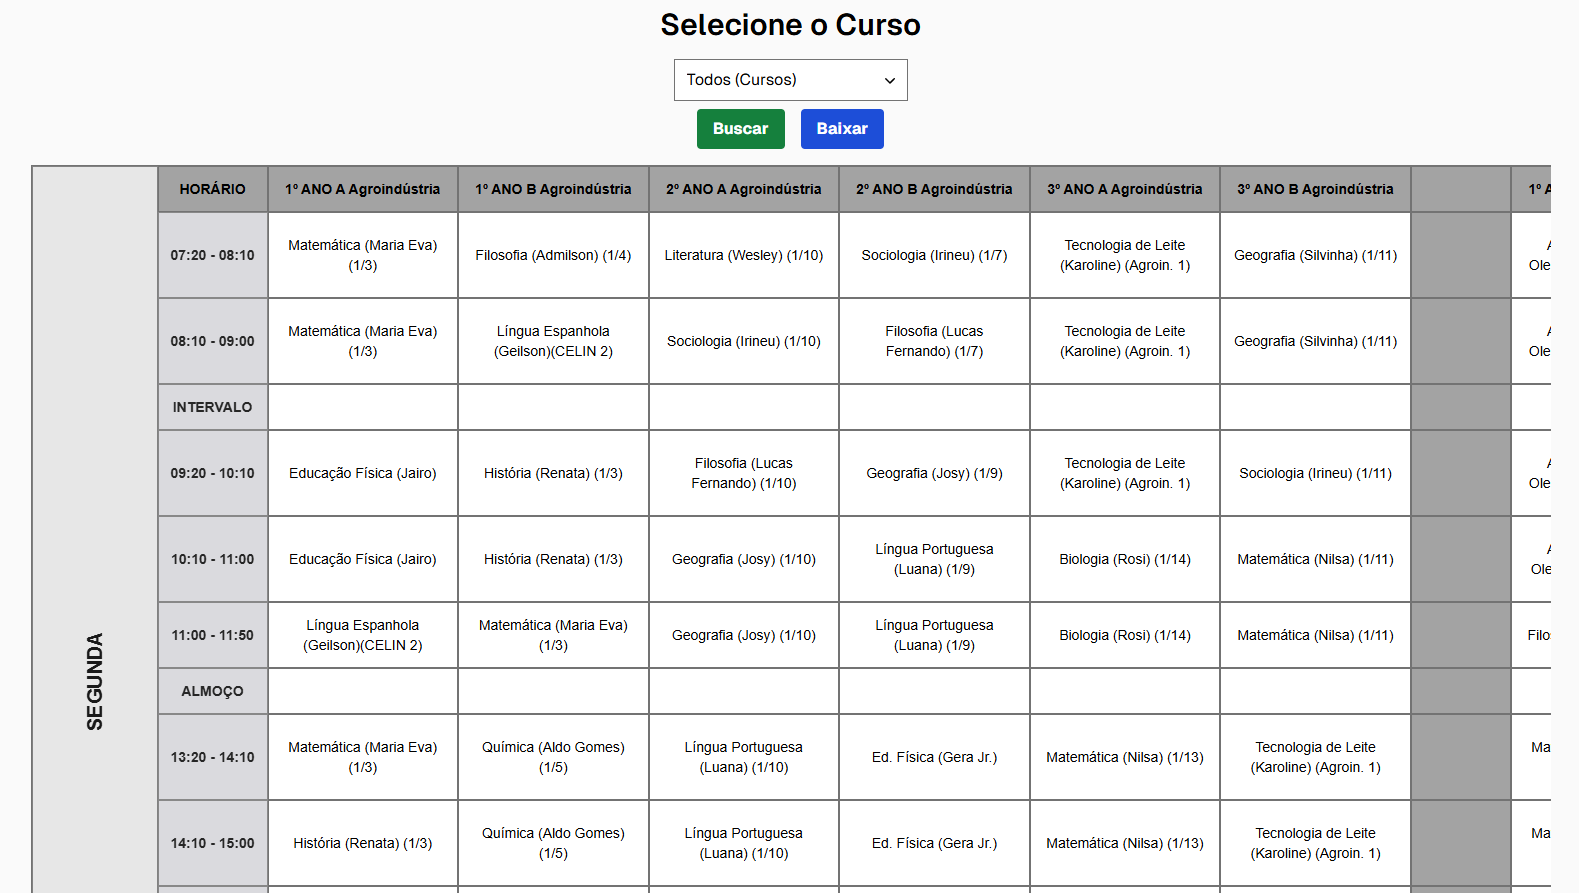
\includegraphics[width=1\textwidth]{Figuras/front-3.png}
    \caption*{Fonte: AUTOR (2025)}
    \label{fig_front_3}
\end{figure}

\begin{figure}[H]
    \centering
    \caption{Tela dos cursos com cursos superiores}
    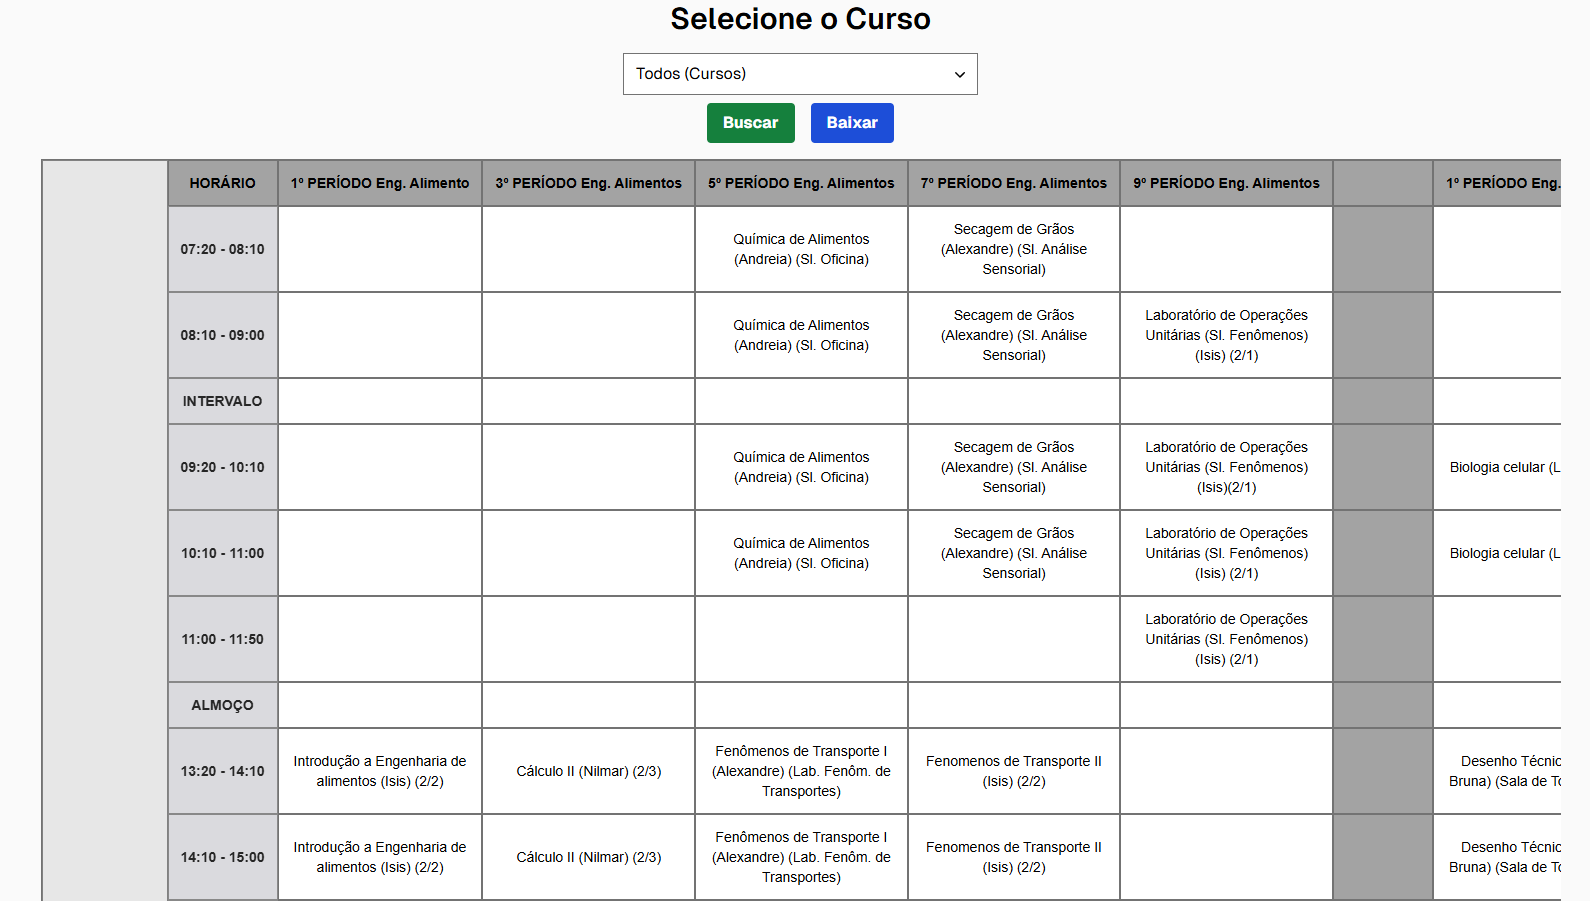
\includegraphics[width=1\textwidth]{Figuras/front-4.png}
    \caption*{Fonte: AUTOR (2025)}
    \label{fig_front_4}
\end{figure}

As Figuras \ref{fig_front_3} e \ref{fig_front_4} detalham, respectivamente, a exibição dos horários para cursos técnicos e superiores.

\begin{figure}[htb]
    \centering
    \caption{Tela dos professores}
    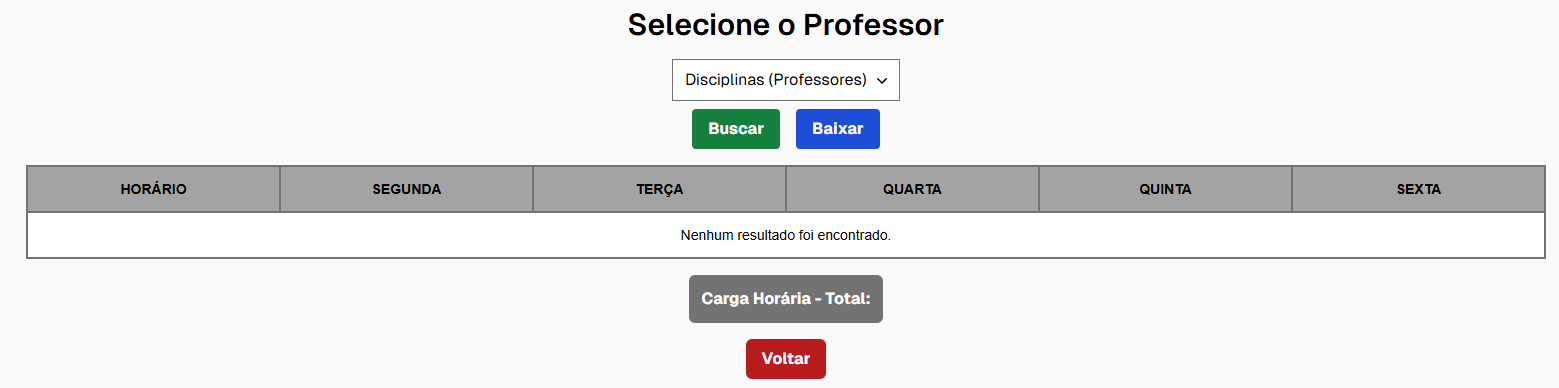
\includegraphics[width=1\textwidth]{Figuras/front-5.png}
    \caption*{Fonte: AUTOR (2025)}
    \label{fig_front_5}
\end{figure}

\begin{figure}[H]
    \centering
    \caption{Tela dos professores com um professor selecionado}
    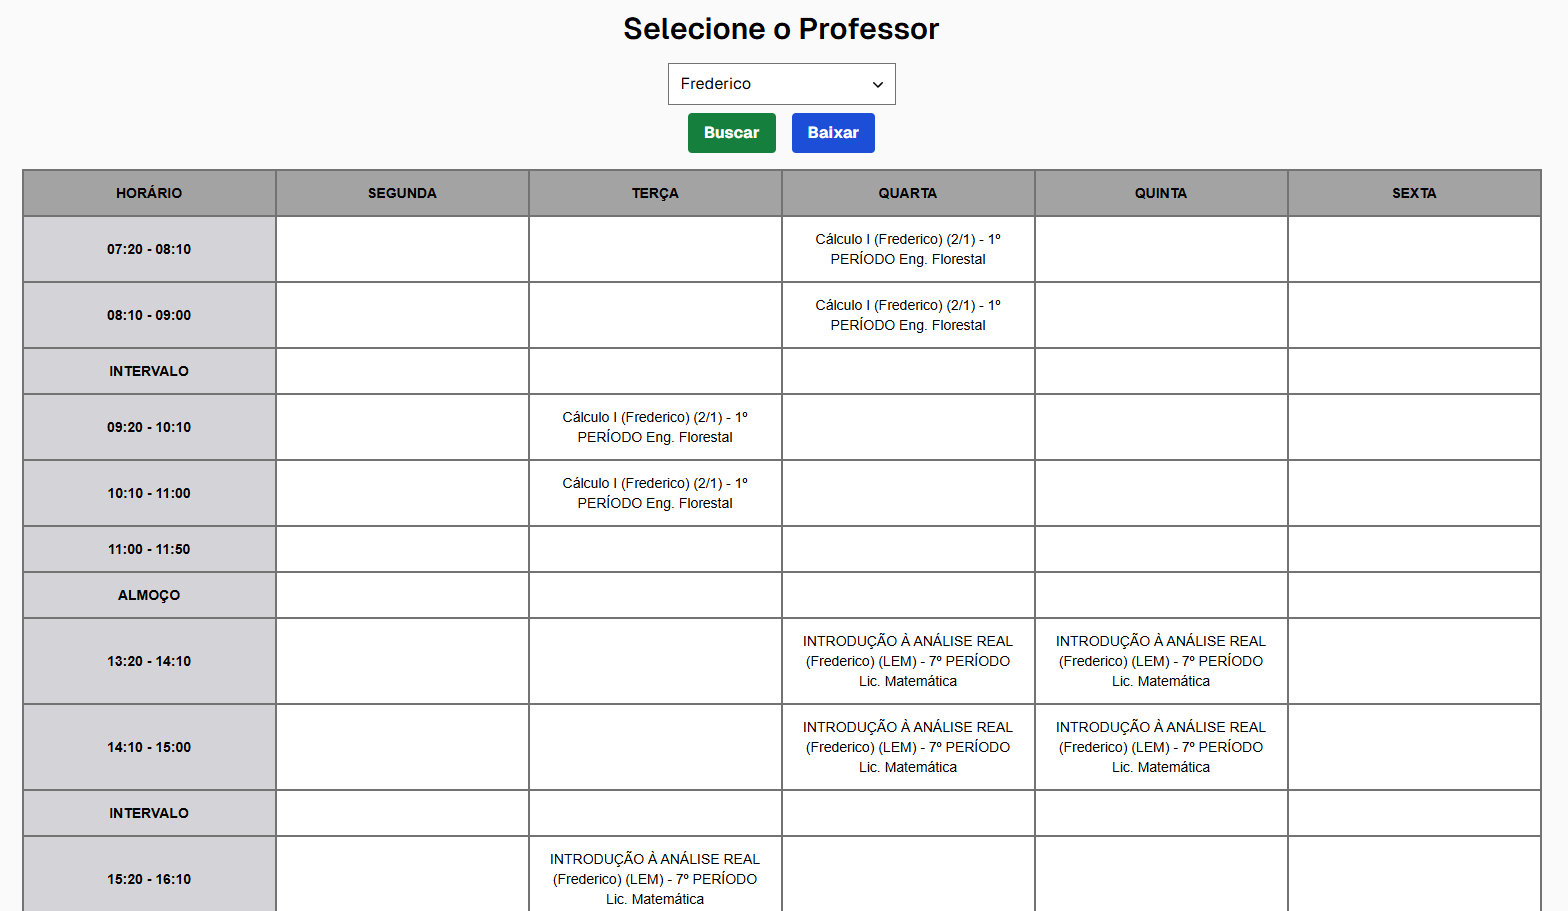
\includegraphics[width=1\textwidth]{Figuras/front-6.png}
    \caption*{Fonte: AUTOR (2025)}
    \label{fig_front_6}
\end{figure}

A Figura \ref{fig_front_5} ilustra a tela dos professores, enquanto a Figura \ref{fig_front_6} exibe um professor selecionado, com seus horários organizados.

\begin{figure}[H]
    \centering
    \caption{Tela das salas}
    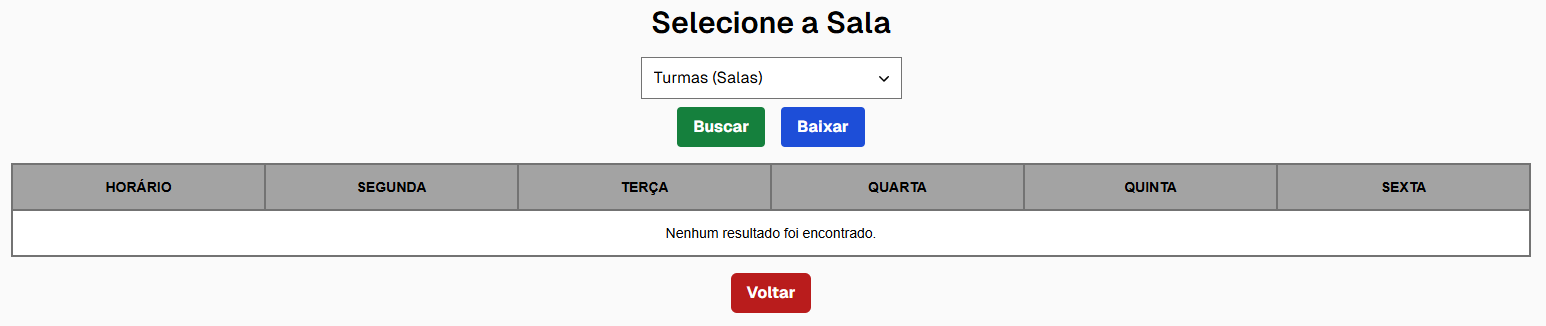
\includegraphics[width=1\textwidth]{Figuras/front-7.png}
    \caption*{Fonte: AUTOR (2025)}
    \label{fig_front_7}
\end{figure}

\begin{figure}[htb]
    \centering
    \caption{Tela das salas com uma sala selecionada}
    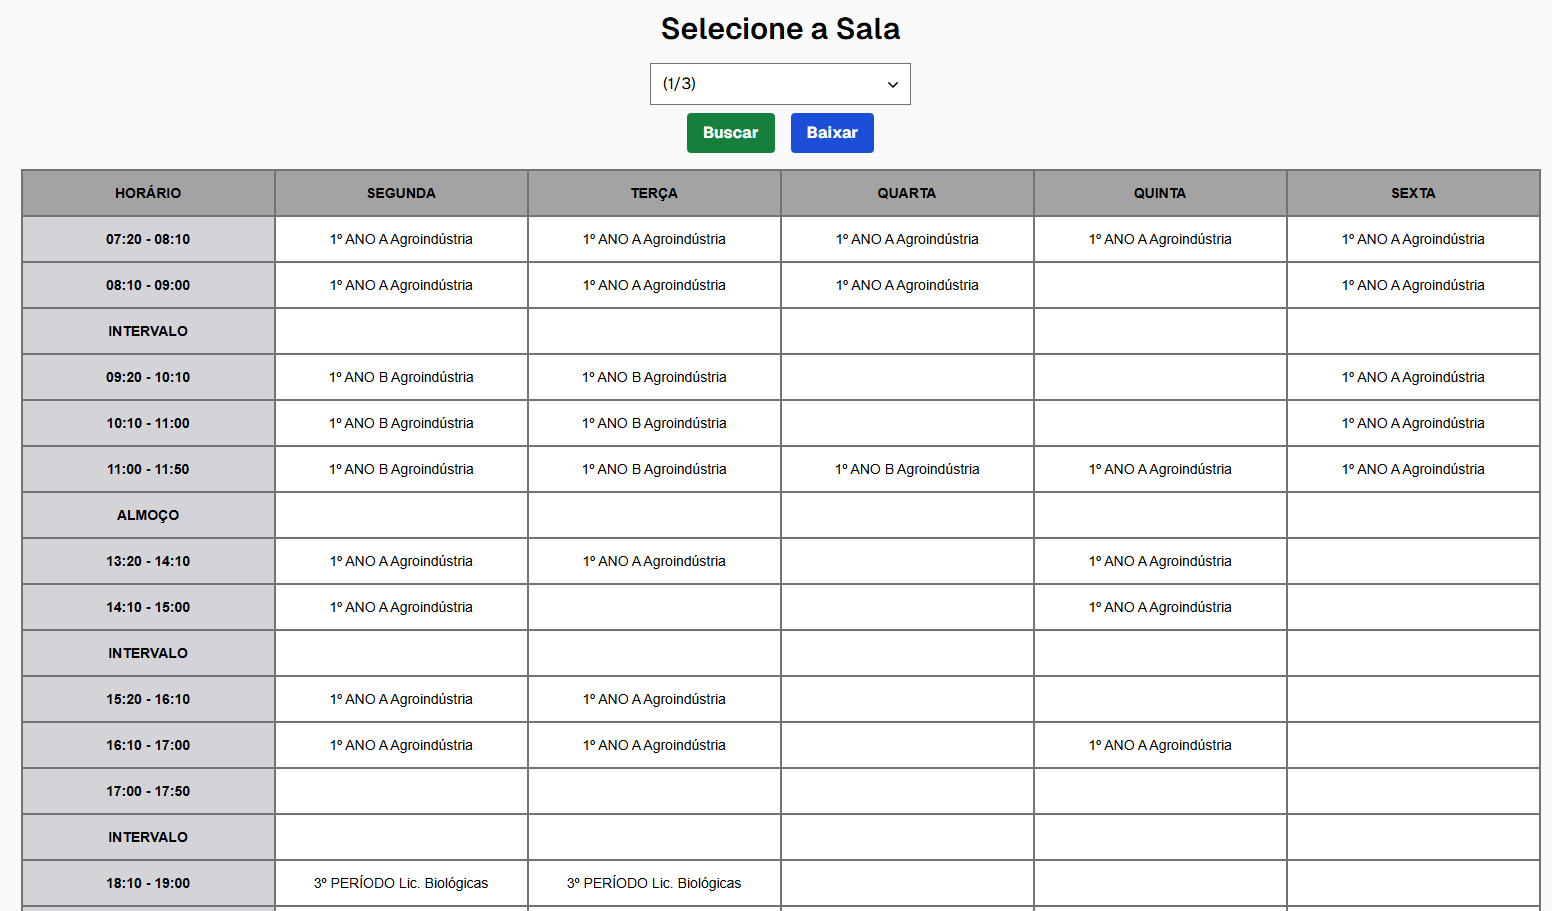
\includegraphics[width=1\textwidth]{Figuras/front-8.png}
    \caption*{Fonte: AUTOR (2025)}
    \label{fig_front_8}
\end{figure}

A Figura \ref{fig_front_7} apresenta a tela das salas e a Figura \ref{fig_front_8} mostra a visualização de uma sala específica com seu cronograma de uso.

\begin{figure}[htb]
    \centering
    \caption{Tela de login para acessar a tela de validação}
    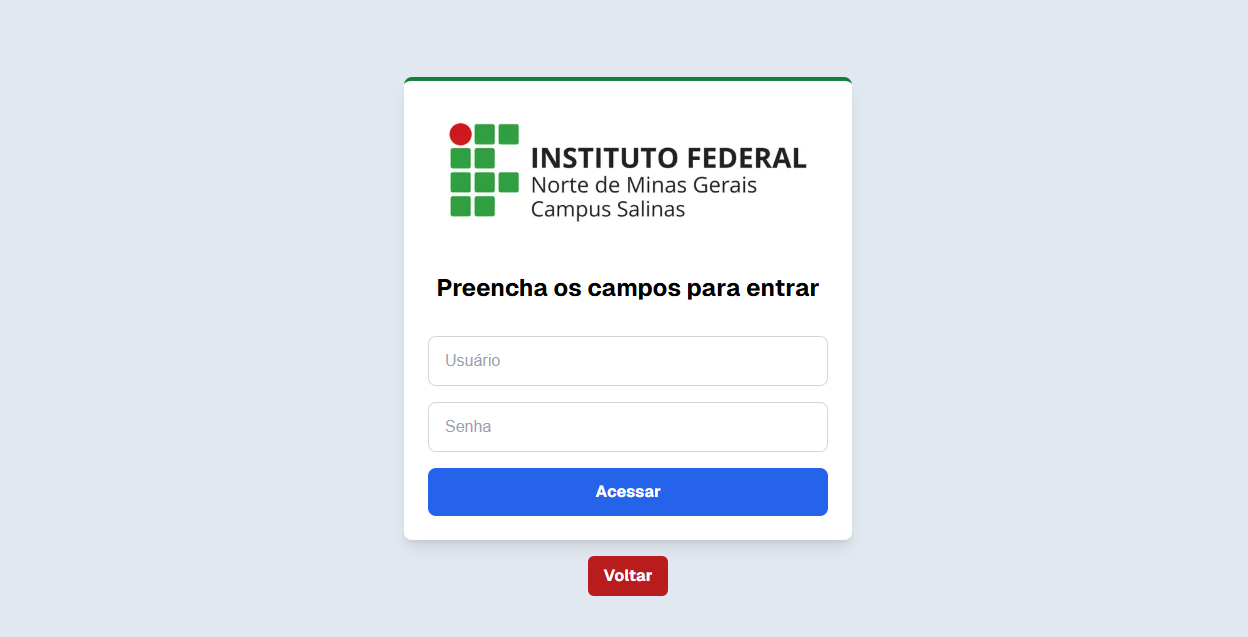
\includegraphics[width=1\textwidth]{Figuras/front-9.png}
    \caption*{Fonte: AUTOR (2025)}
    \label{fig_front_9}
\end{figure}

\begin{figure}[H]
    \centering
    \caption{Tela de validação}
    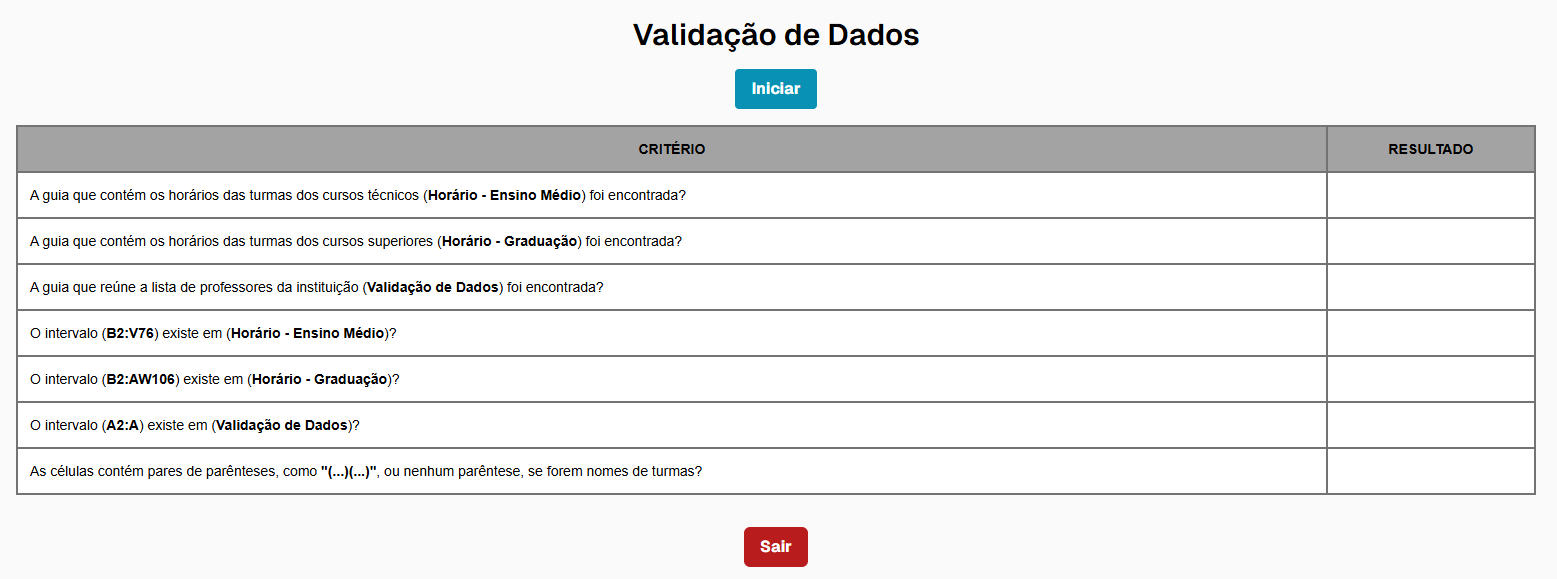
\includegraphics[width=1\textwidth]{Figuras/front-10.png}
    \caption*{Fonte: AUTOR (2025)}
    \label{fig_front_10}
\end{figure}

Já a Figura \ref{fig_front_9} traz a tela de login para acessar a área de validação de dados, e a Figura \ref{fig_front_10} mostra a tela de validação.

\begin{figure}[htb]
    \centering
    \caption{Sistema que exibe os locais do instituto}
    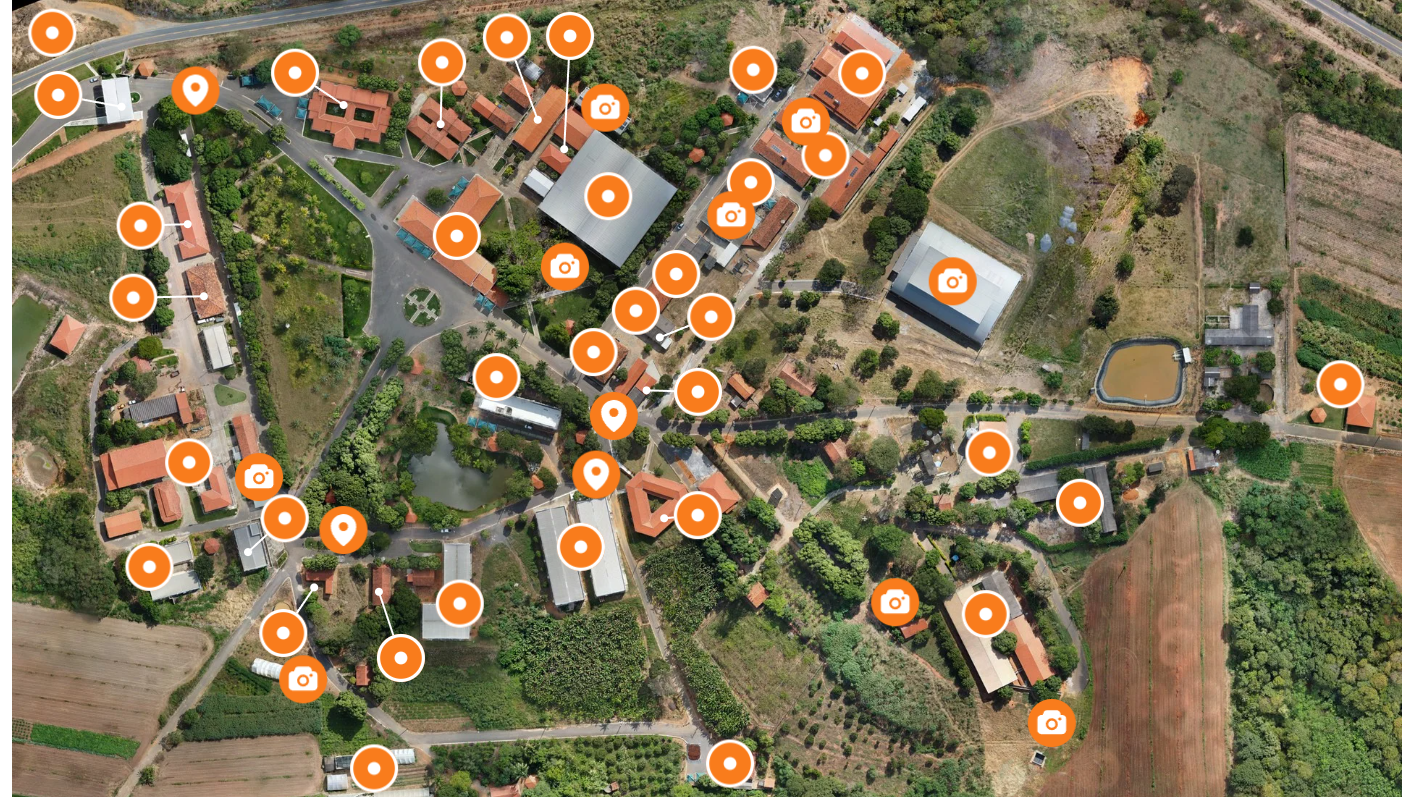
\includegraphics[width=1\textwidth]{Figuras/front-11.png}
    \caption*{Fonte: AUTOR (2025)}
    \label{fig_front_11}
\end{figure}

\begin{figure}[H]
    \centering
    \caption{Sistema de reserva de horários}
    
\includegraphics[width=1\textwidth]{Figuras/front-12.png}
    \caption*{Fonte: AUTOR (2025)}
    \label{fig_front_12}
\end{figure}

\begin{figure}[htb]
    \centering
    \caption{Sistema de gerenciamento de reserva de salas}
    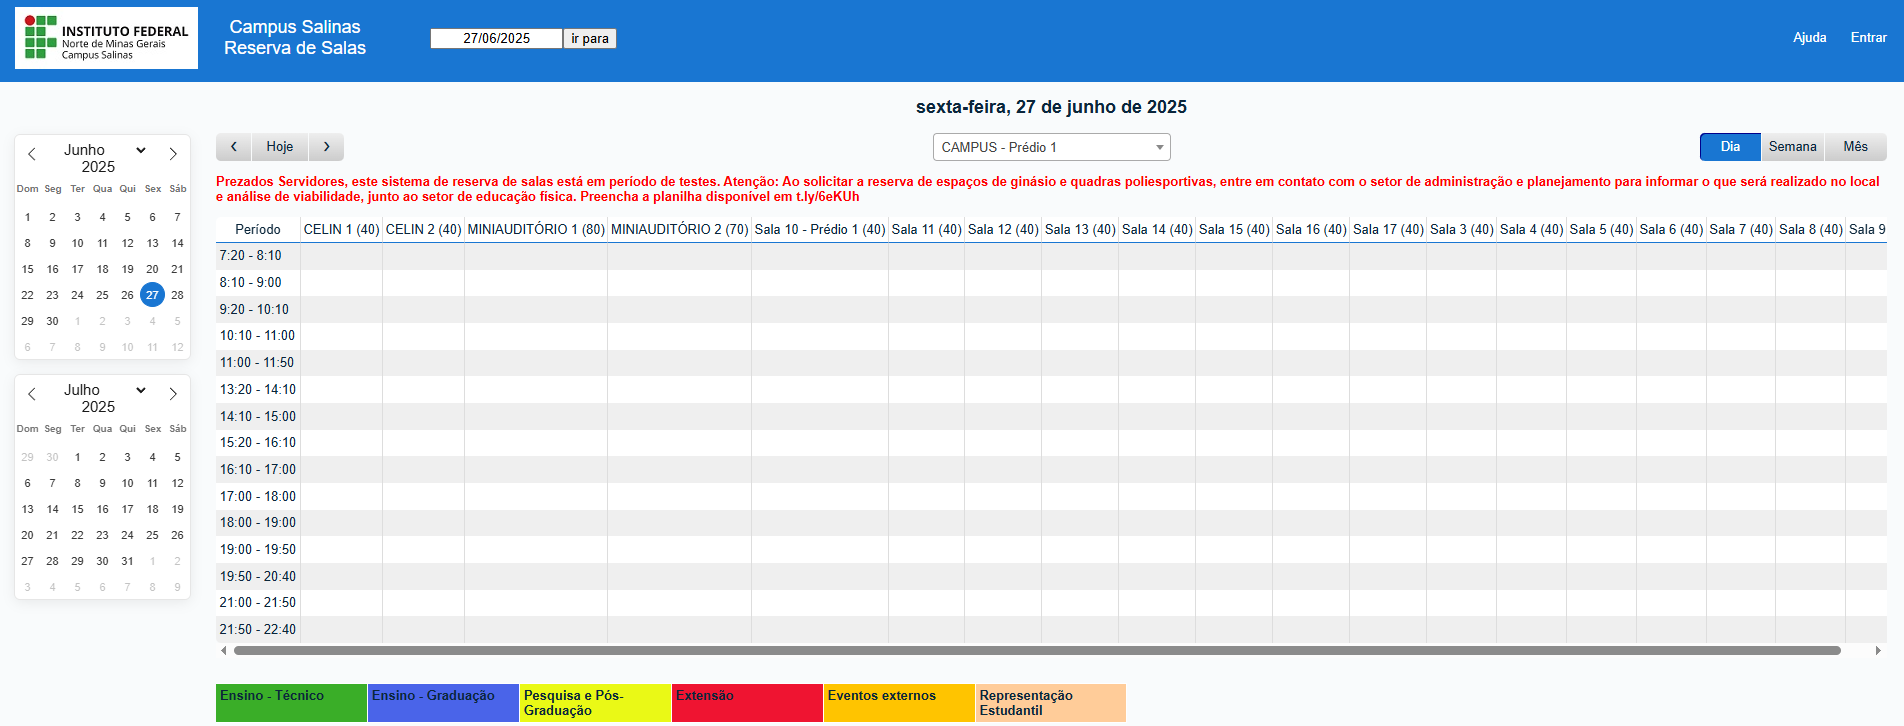
\includegraphics[width=1\textwidth]{Figuras/front-13.png}
    \caption*{Fonte: AUTOR (2025)}
    \label{fig_front_13}
\end{figure}

Por fim, as Figuras \ref{fig_front_11}, \ref{fig_front_12} e \ref{fig_front_13} ilustram os sistemas externos integrados à plataforma, incluindo a visualização de locais do instituto, o sistema de reserva de horários e o gerenciamento de reservas de salas. Esses sistemas, embora estejam acessíveis a partir da plataforma desenvolvida, não estão incluídos no escopo desse trabalho.

\subsection{Estrutura do Front-end}

A estrutura do front-end está organizada de forma modular, visando clareza, manutenção facilitada e reutilização de código. Na Figura \ref{fig_front_14}, destacam-se os principais elementos:

\begin{figure}[htb]
    \centering
    \caption{Estrutura do front-end}
    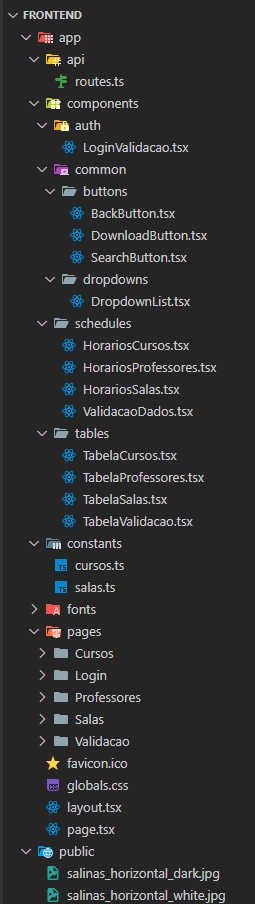
\includegraphics[width=0.3\textwidth]{Figuras/front-14.png}
    \caption*{Fonte: AUTOR (2025)}
    \label{fig_front_14}
\end{figure}

\begin{itemize}
    \item api: pasta responsável por buscar dados da planilha por meio de requisições, contando com o arquivo routes.ts, que gerencia essas chamadas e contém a variável de ambiente para comunicação com o back-end.
    \item components: pasta que centraliza os componentes do sistema, subdividida em:
    \begin{itemize}
        \item auth: pasta responsável pelo controle de autenticação, incluindo o arquivo LoginValidacao.tsx, que verifica as credenciais de login antes de entrar na tela de validação.
        \item common: pasta destinada a componentes reutilizáveis, contendo:
        \begin{itemize}
            \item buttons: reúne botões de ação como BackButton.tsx para retorno, DownloadButton.tsx para download de tabelas e SearchButton.tsx para busca de horários.
             \item dropdowns: responsável pelas listas suspensas, como o arquivo DropdownList.tsx, utilizado para seleção de cursos, professores ou salas.
        \end{itemize}
        \item schedules: pasta com componentes independentes para exibição de horários organizados por tipo de consulta, como HorariosCursos.tsx, HorariosProfessores.tsx e HorariosSalas.tsx, que apresentam uma lista suspensa para seleção e uma tabela com os horários correspondentes, e ValidacaoDados.tsx, que exibe a tabela com os resultados da validação da planilha dos horários.
        \item tables: pasta com componentes independentes das tabelas com os dados, incluindo TabelaCursos.tsx, TabelaProfessores.tsx, TabelaSalas.tsx e TabelaValidacao.tsx.
    \end{itemize}
    \item constants: pasta responsável por definir as listas de cursos e salas disponíveis, armazenadas nos arquivos cursos.ts e salas.ts.
    \item pages: organiza as rotas da aplicação, com páginas específicas para cursos, professores, salas, login e validação.
    \item globals.css: arquivo de estilos globais aplicados em toda a interface.
    \item layout.tsx: define a estrutura geral de layout e permite a edição de metadados de forma centralizada.
    \item page.tsx: página inicial que exibe o menu principal com opções de botões de horários e outros serviços.
    \item public: pasta com imagens do logotipo institucional do IFNMG Campus Salinas, disponibilizadas tanto na versão padrão quanto na versão em preto e branco.
\end{itemize}

\subsection{Funcionalidades do Front-end}

\begin{itemize}
    \item \textbf{Modo escuro}: adapta automaticamente o tema da aplicação entre claro ou escuro, de acordo com a configuração do navegador, oferecendo maior conforto visual aos usuários. Conforme mostrado na Figura \ref{fig_front_15}.

    \begin{figure}[htb]
        \centering
        \caption{Modo escuro}
        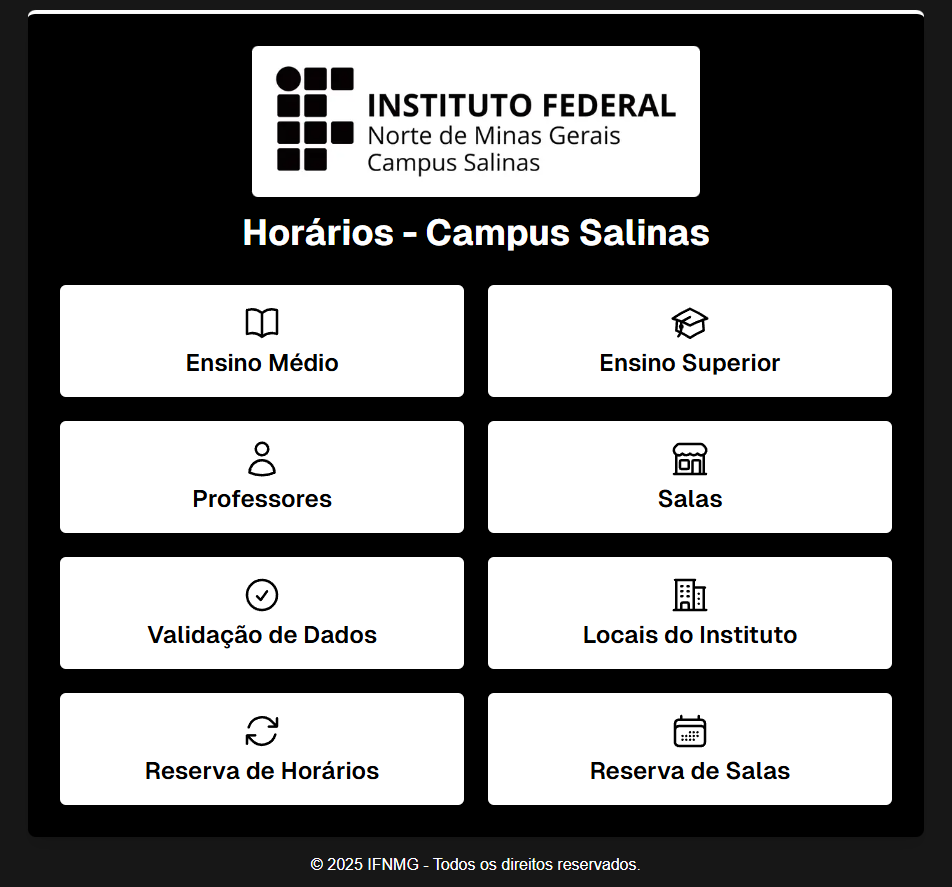
\includegraphics[width=1\textwidth]{Figuras/front-15.png}
        \caption*{Fonte: AUTOR (2025)}
        \label{fig_front_15}
    \end{figure}

    \item \textbf{Responsividade}: garante que a interface funcione bem tanto em dispositivos móveis quanto em desktops, mantendo a usabilidade e a organização dos elementos. Conforme mostrado na Figura \ref{fig_front_16}.

    \begin{figure}[H]
        \centering
        \caption{Responsividade}
        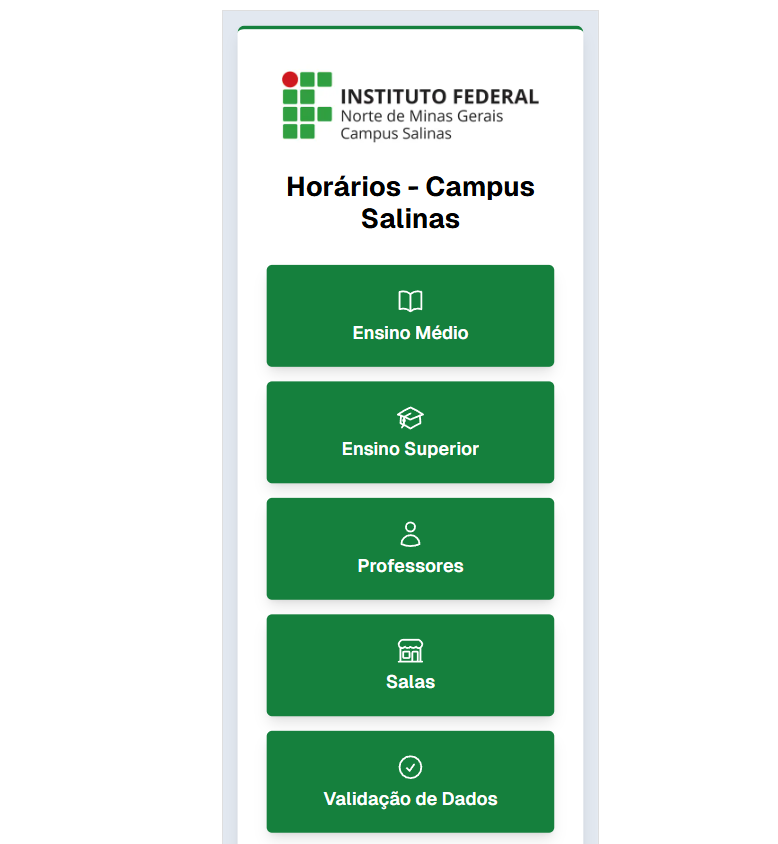
\includegraphics[width=0.7\textwidth]{Figuras/front-16.png}
        \caption*{Fonte: AUTOR (2025)}
        \label{fig_front_16}
    \end{figure}
    
    \item \textbf{Busca de horários de cursos}: possibilita consultar os horários dos cursos técnicos e superiores, exibindo os dias e horários de segunda a sexta-feira. Apresentado na Figura \ref{fig_front_17}.

    \begin{figure}[htb]
        \centering
        \caption{Busca de horários de cursos}
        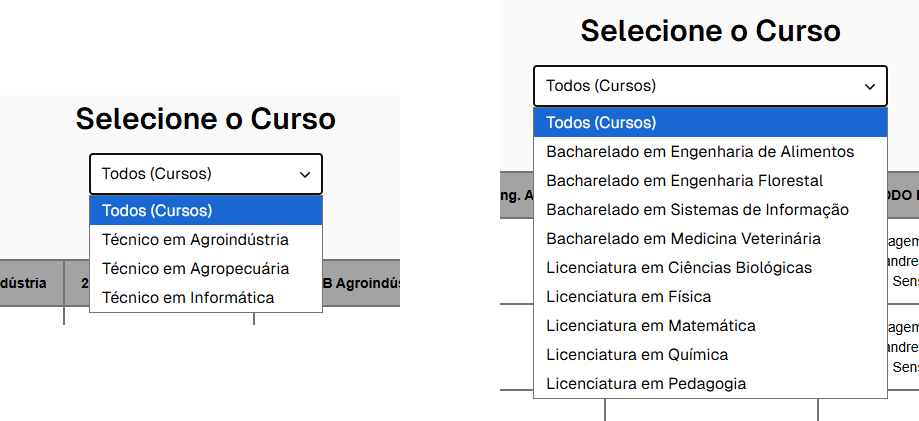
\includegraphics[width=0.7\textwidth]{Figuras/front-17.png}
        \caption*{Fonte: AUTOR (2025)}
        \label{fig_front_17}
    \end{figure}
    
    \item \textbf{Busca de horários de professores}: permite selecionar um professor em uma lista suspensa e visualizar os horários de segunda a sexta-feira. Ilustrado na Figura \ref{fig_front_18}.

    \begin{figure}[htb]
        \centering
        \caption{Busca de horários de professores}
        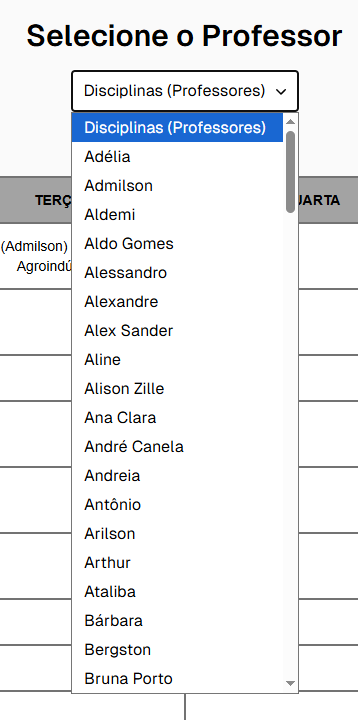
\includegraphics[width=0.6\textwidth]{Figuras/front-18.png}
        \caption*{Fonte: AUTOR (2025)}
        \label{fig_front_18}
    \end{figure}
    
    \item \textbf{Busca de horários de salas}: permite selecionar uma sala em uma lista suspensa e visualizar os horários de ocupação de segunda a sexta-feira. Conforme mostrado na Figura \ref{fig_front_19}.

    \begin{figure}[htb]
        \centering
        \caption{Busca de horários de salas}
        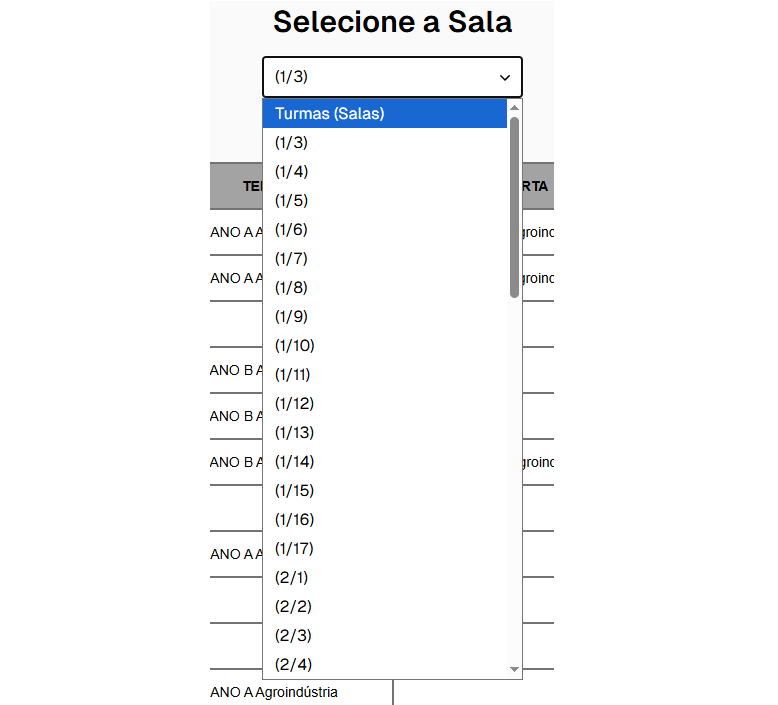
\includegraphics[width=0.5\textwidth]{Figuras/front-19.png}
        \caption*{Fonte: AUTOR (2025)}
        \label{fig_front_19}
    \end{figure}
    
    \item \textbf{Download em PDF}: permite o usuário salvar a tabela dos horários em um arquivo no formato PDF, facilitando o acesso offline às informações. Conforme mostrado na Figura \ref{fig_front_20}.

    \begin{figure}[htb]
        \centering
        \caption{Download em PDF}
        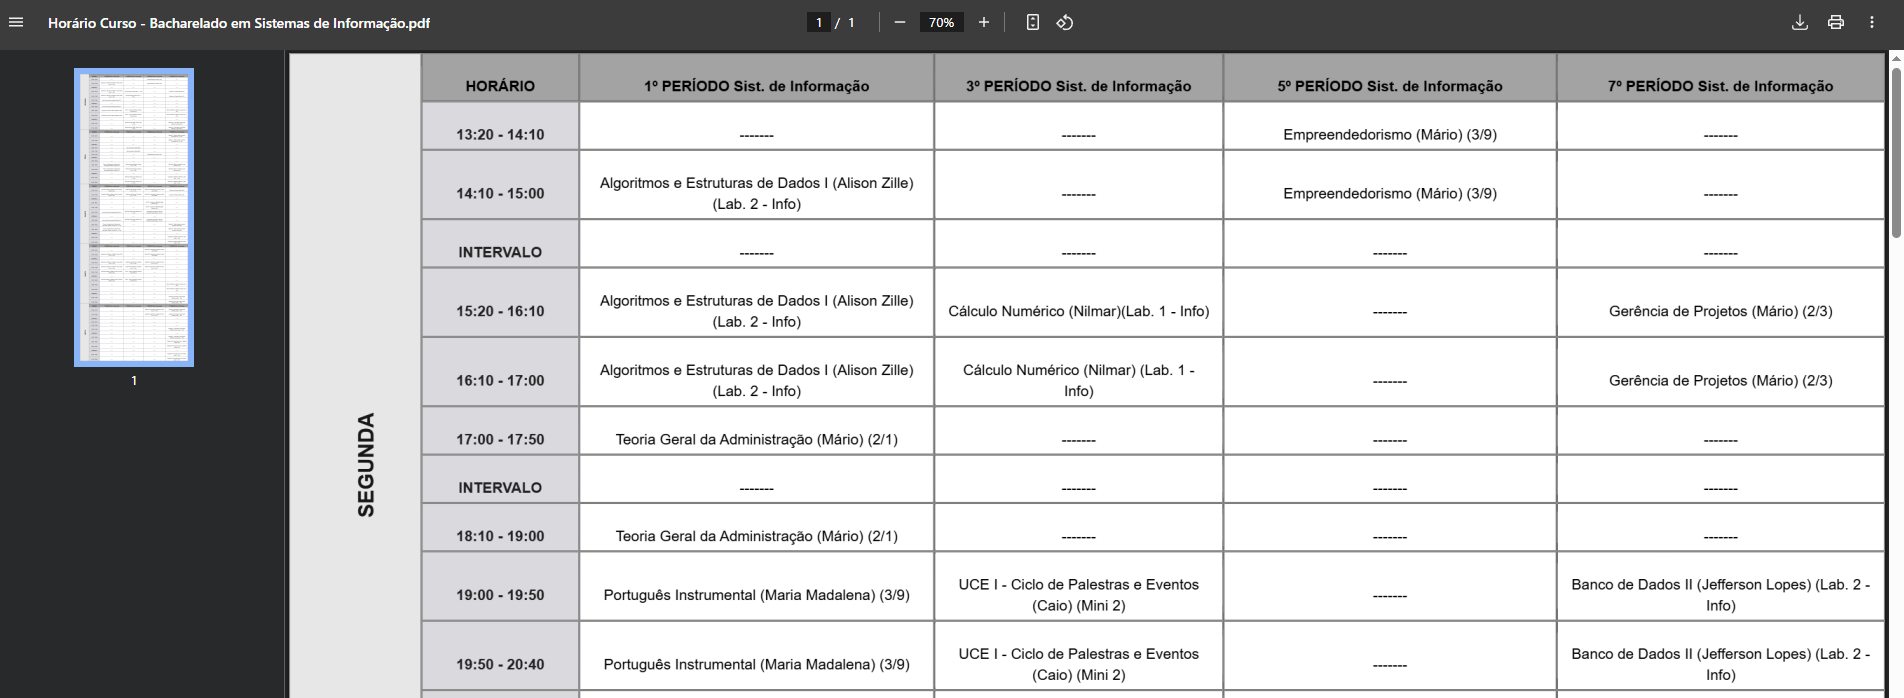
\includegraphics[width=0.9\textwidth]{Figuras/front-20.png}
        \caption*{Fonte: AUTOR (2025)}
        \label{fig_front_20}
    \end{figure}
    
    \item \textbf{Tela de login}: restringe o acesso à tela de validação de dados apenas aos administradores, por meio de autenticação com usuário e senha. Ver Figura \ref{fig_front_21}.

    \begin{figure}[htb]
        \centering
        \caption{Tela de login com credenciais incorretas}
        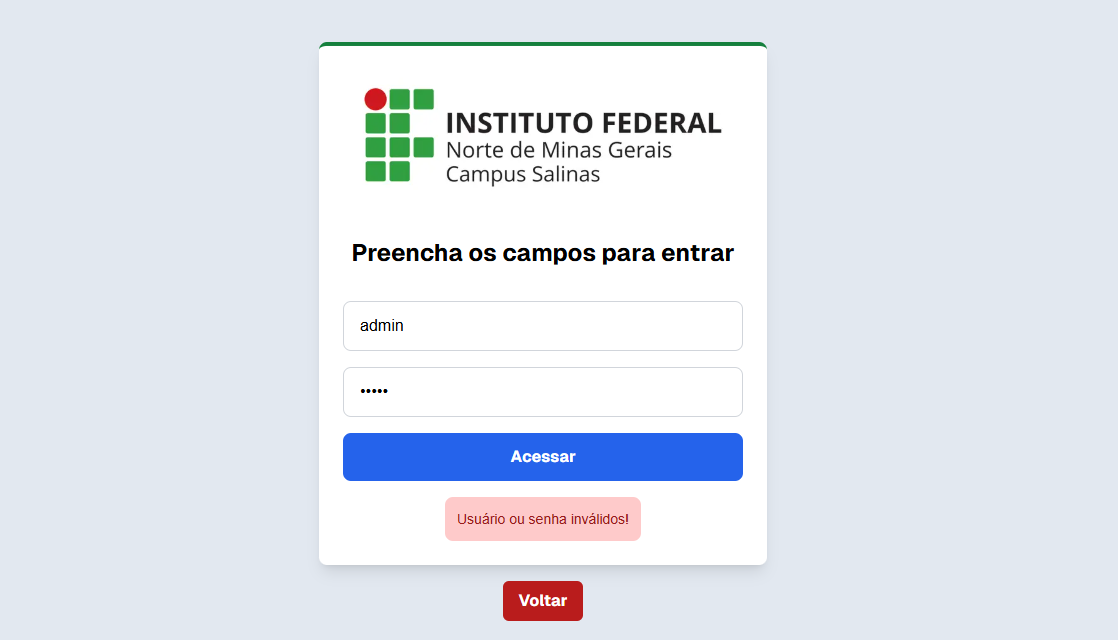
\includegraphics[width=0.8\textwidth]{Figuras/front-21.png}
        \caption*{Fonte: AUTOR (2025)}
        \label{fig_front_21}
    \end{figure}
    
    \item \textbf{Tela de validação}: exibe os resultados da verificação da planilha de horários, apresentando uma tabela com indicadores de conformidade (SIM ou NÃO) e validando: (melhorar)
    \begin{itemize}
        \item a presença das guias Horário - Ensino Médio, Horário - Graduação e Validação de Dados;
        \item a existência dos intervalos de células (B2:V76), (B2:AW106) e (A2:A);
        \item a formatação correta dos nomes, verificando se contêm os parênteses exigidos para turmas e professores. Se forem encontradas inconsistências, a tela exibe as células problemáticas, informando a guia, coluna e linha correspondentes. Ilustrado na Figura \ref{fig_front_22}.
    \end{itemize}

    \begin{figure}[htb]
        \centering
        \caption{Tela de validação com resultados}
        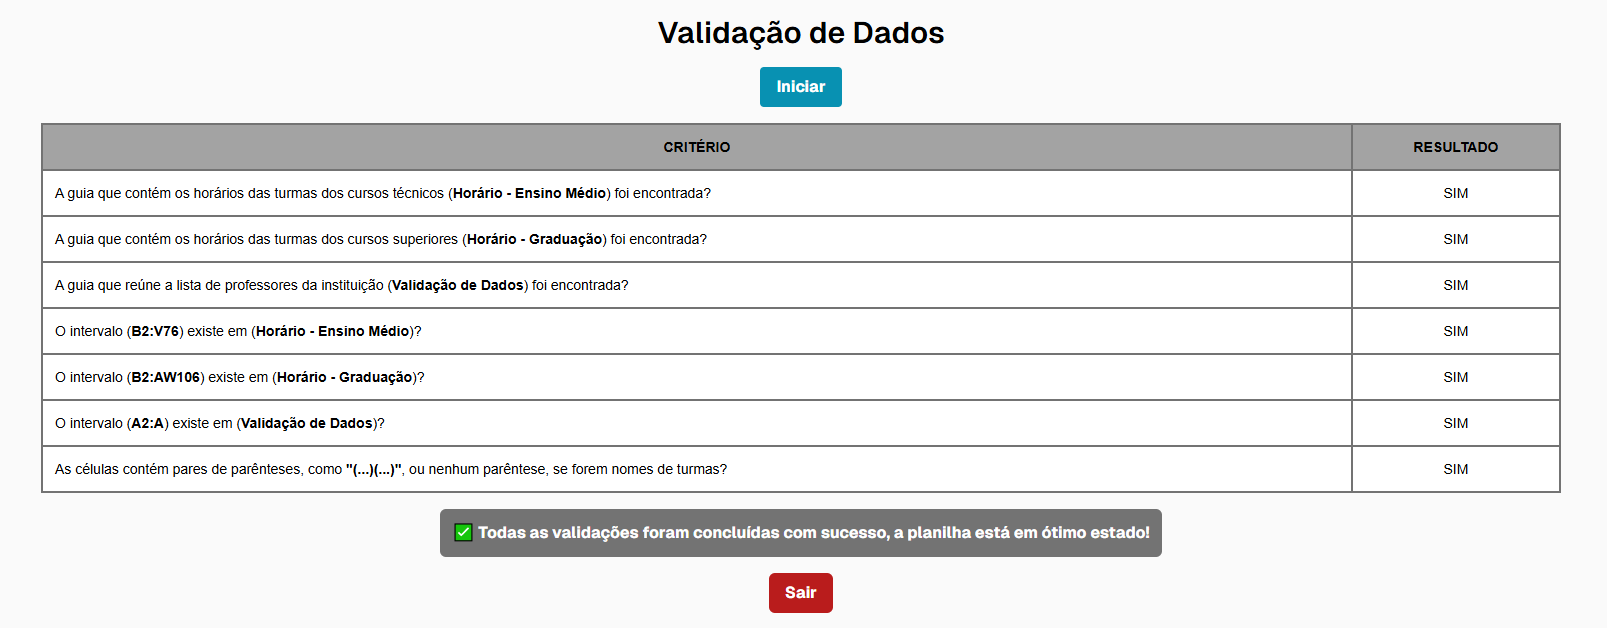
\includegraphics[width=1\textwidth]{Figuras/front-22.png}
        \caption*{Fonte: AUTOR (2025)}
        \label{fig_front_22}
    \end{figure}
\end{itemize}

\section{Back-end}

\subsection{Google Sheets como Banco de Dados}

O sistema utiliza duas planilhas hospedadas no Google Sheets. A primeira planilha contém duas guias com os horários acadêmicos e a uma guia com a lista dos professores disponíveis, conforme apresentado a seguir:

\begin{figure}[H]
    \centering
    \caption{Horário - Ensino Médio}
    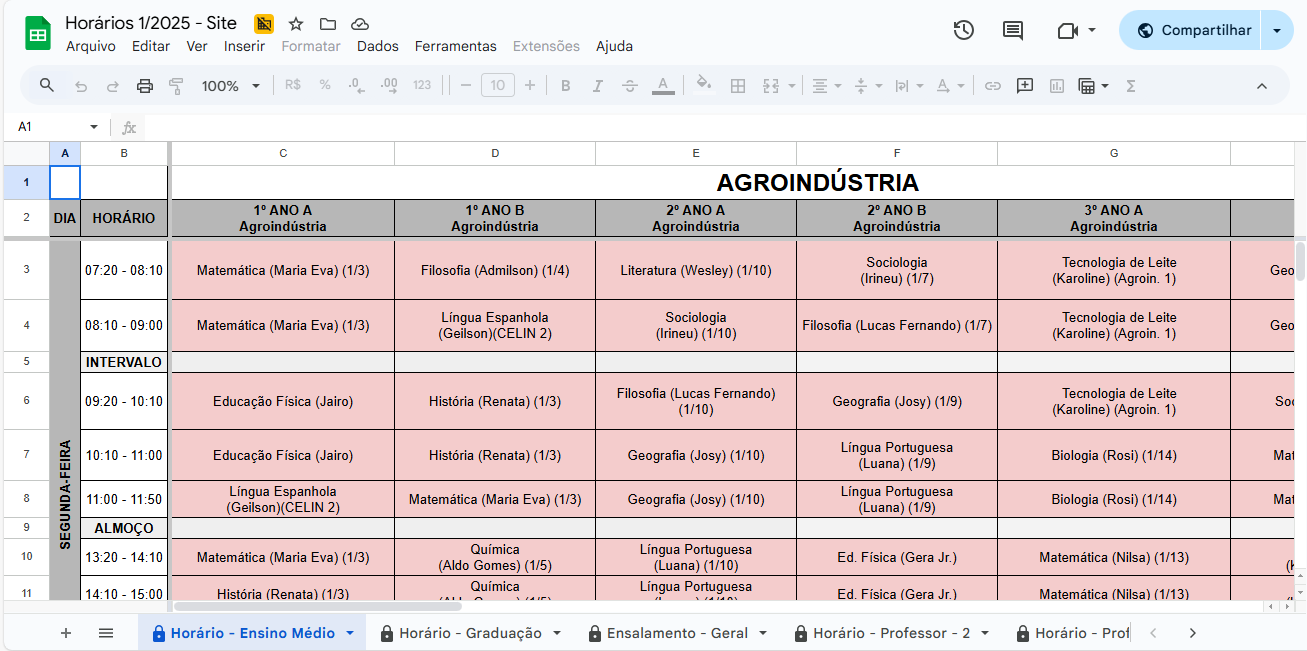
\includegraphics[width=0.9\textwidth]{Figuras/plan-1.png}
    \caption*{Fonte: AUTOR (2025)}
    \label{fig_plan_1}
\end{figure}

A Figura \ref{fig_plan_1} mostra a guia que contém os horários das turmas dos cursos técnicos, distribuídos no intervalo de células B2:V76.

\begin{figure}[htb]
    \centering
    \caption{Horário - Graduação}
    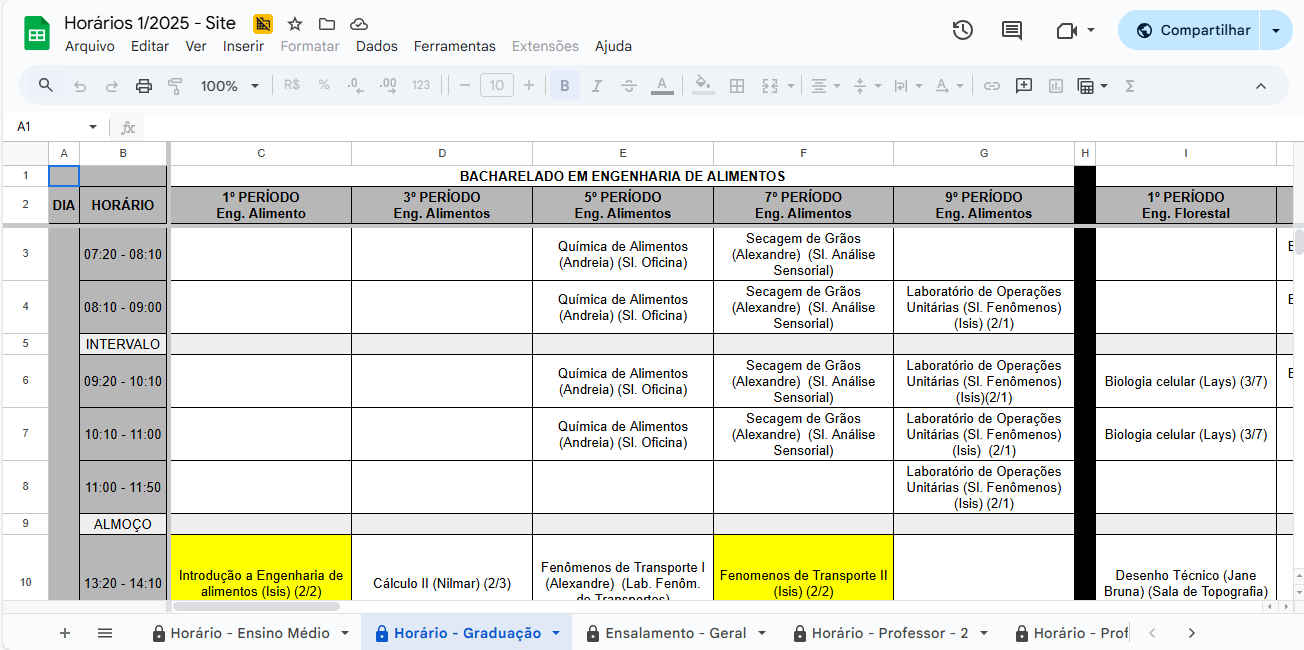
\includegraphics[width=0.9\textwidth]{Figuras/plan-2.png}
    \caption*{Fonte: AUTOR (2025)}
    \label{fig_plan_2}
\end{figure}

A Figura \ref{fig_plan_2} mostra a guia que contém os horários das turmas dos cursos superiores, distribuídos no intervalo de células B2:AW106.

\begin{figure}[H]
    \centering
    \caption{Validação de Dados}
    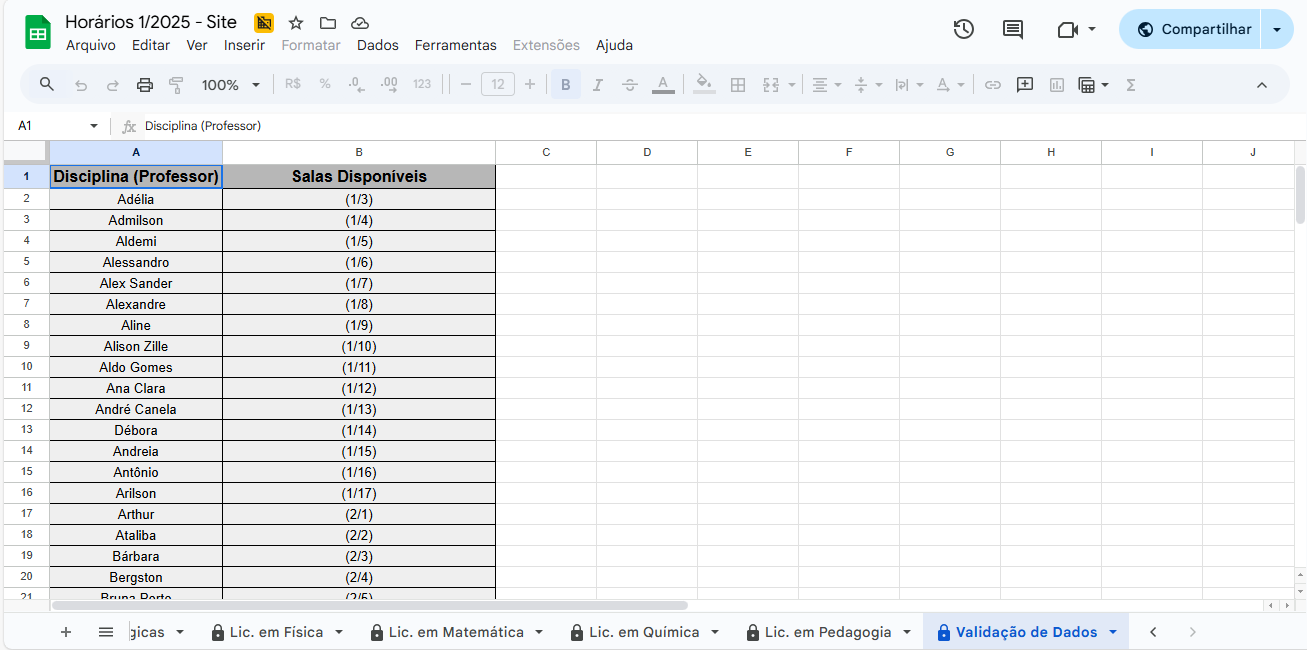
\includegraphics[width=0.9\textwidth]{Figuras/plan-3.png}
    \caption*{Fonte: AUTOR (2025)}
    \label{fig_plan_3}
\end{figure}

A Figura \ref{fig_plan_3}, mostra a guia que reúne a lista de professores da instituição, distribuídos no intervalo de células A2:A.

A segunda planilha contém uma guia com as credenciais de login necessárias para autenticação:

\begin{figure}[htb]
    \centering
    \caption{Login}
    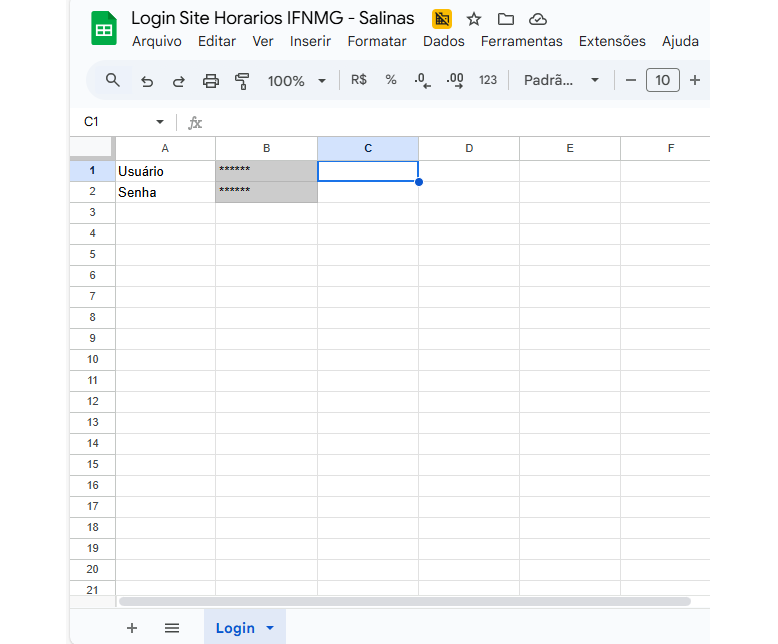
\includegraphics[width=0.75\textwidth]{Figuras/plan-4.png}
    \caption*{Fonte: AUTOR (2025)}
    \label{fig_plan_4}
\end{figure}

A Figura \ref{fig_plan_4} mostra a guia da planilha com as credenciais de login para acessar a tela de validação de dados, contendo os campos de usuário e senha, distribuídos no intervalo de células B1:B2.

\subsection{Desenvolvimento do Back-end}

O back-end foi desenvolvido utilizando o framework Spring Boot, escolhido por sua robustez, flexibilidade e ampla adoção no mercado. Essa tecnologia possibilitou integrar de forma segura a API do Google Sheets, garantindo a leitura dos dados necessários para o funcionamento da plataforma e enviando essas informações ao front-end de maneira estruturada e confiável. Todo o processo priorizou simplicidade na configuração e facilidade de manutenção, permitindo atender às demandas do projeto com eficiência. O código está disponível no repositório do projeto em \url{https://github.com/Tomaz5556/Horarios-IFNMG-Salinas/tree/main/backend}.

\subsection{Estrutura do Back-end}

A estrutura do back-end está organizada seguindo o padrão arquitetural MVC, o que favorece a separação de responsabilidades, facilita a manutenção e a evolução do sistema. Na Figura \ref{fig_back_1}, destacam-se os principais elementos do projeto:

\begin{figure}[htb]
    \centering
    \caption{Estrutura do back-end}
    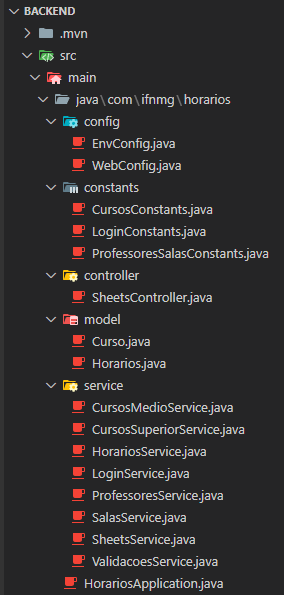
\includegraphics[width=0.85\textwidth]{Figuras/back-1.png}
    \caption*{Fonte: AUTOR (2025)}
    \label{fig_back_1}
\end{figure}

\begin{itemize}
    \item config: pacote para armazenar classes de configuração do sistema, como a EnvConfig.java, que define as variáveis de ambiente, e a WebConfig.java, responsável por ajustes na configuração do Spring Boot, incluindo a definição do CORS. Um mecanismo que define quais origens externas podem se comunicar com a API, permitindo uma integração segura entre o front-end e o back-end, mesmo em domínios diferentes.
    \item constants: pacote para centralizar valores fixos e listas, contendo as classes CursosConstants.java, LoginConstants.java e ProfessoresSalasConstants.java, que mantêm os dados de cursos, professores, salas e credenciais de login.
    \item controller: pacote para controlar as requisições recebidas e encaminhá-las para os serviços adequados, abrigando a classe SheetsController.java, que gerencia as rotas da aplicação.
    \item model: pacote para definir as classes de domínio que representam a estrutura dos dados, como Curso.java e Horarios.java, que servem de modelo para a manipulação das informações obtidas do Google Sheets.
    \item service: pacote para concentrar as regras de negócio e a comunicação com a API do Google Sheets, incluindo as classes CursosMedioService.java, CursosSuperiorService.java, HorariosService.java, LoginService.java, ProfessoresService.java, SalasService.java, SheetsService.java e ValidacoesService.java.
    \item HorariosApplication.java: classe principal que executa a aplicação Spring Boot e carrega as configurações do sistema.
\end{itemize}

\subsection{Funcionalidades do Back-end}

\begin{itemize}
    \item \textbf{Estabelecer a conexão com a API do Google Sheets}: para coletar os dados das planilhas utilizadas como banco de dados. Essa função é executada pela classe SheetsService, que gerencia a integração entre o back-end e o serviço do Google, possibilitando o acesso dinâmico e estruturado às informações necessárias para o funcionamento da plataforma.
    
    \begin{figure}[H]
        \centering
        \caption{SheetsService.java}
        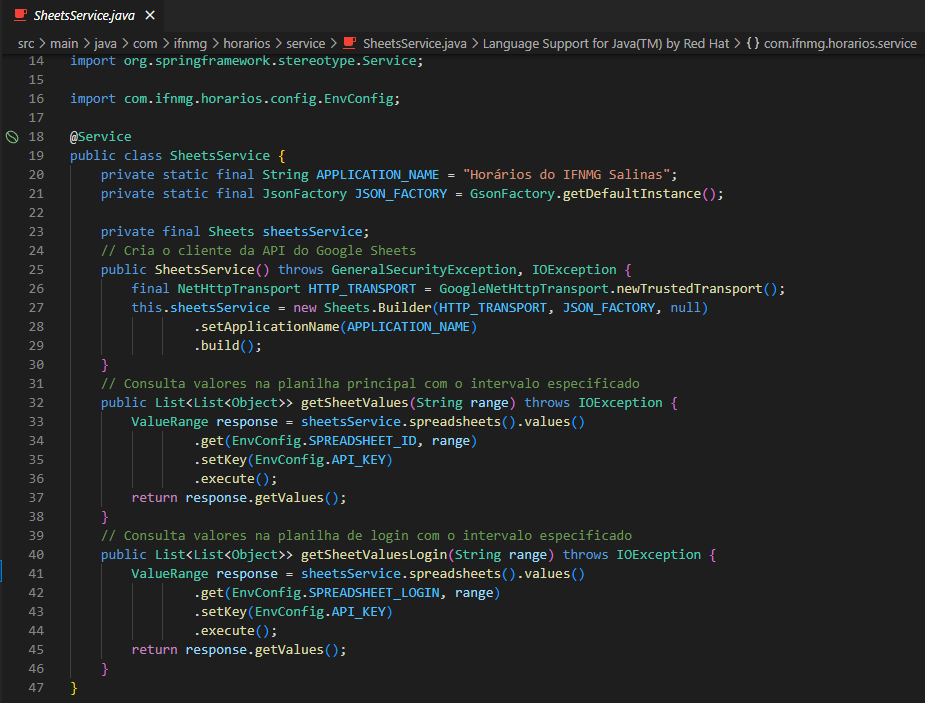
\includegraphics[width=1\textwidth]{Figuras/back-2.png}
        \caption*{Fonte: AUTOR (2025)}
        \label{fig_back_2}
    \end{figure}
    
    A Figura \ref{fig_back_2} mostra a classe SheetsService.java. A seguir, estão descritas suas principais funcionalidades:

    \begin{itemize}
        \item \textbf{Constantes}: APPLICATION\_NAME e JSON\_FACTORY são utilizadas para configurar a instância da API do Google Sheets. O nome da aplicação é definido para identificação no console da API, e o JsonFactory especifica o formato de serialização dos dados trafegados entre o back-end e o serviço do Google.
        \item \textbf{Construtor SheetsService()}: Responsável por configurar a instância do cliente da API do Google Sheets, que é armazenada no atributo sheetsService. Para isso, é utilizada uma conexão segura, criada com GoogleNetHttpTransport, garantindo uma comunicação autenticada e confiável entre o sistema e a API.
        \item \textbf{Método getSheetValues(String range)}: Realiza a leitura dos dados da planilha principal, onde estão os horários acadêmicos, com base no intervalo informado pelo parâmetro range. O método utiliza duas variáveis de ambiente:
        \begin{itemize}
            \item \textit{EnvConfig.SPREADSHEET\_ID}: ID da planilha com os horários acadêmicos.
            \item \textit{EnvConfig.API\_KEY}: chave de API do Google Sheets.
        \end{itemize}
        \item \textbf{Método getSheetValuesLogin(String range)}: Realiza a leitura dos dados da planilha de login, com base no intervalo informado pelo parâmetro range. Esse método é executado antes do acesso à tela de validação de dados, sendo responsável por autenticar o usuário na tela de login. As variáveis de ambiente utilizadas são:
        \begin{itemize}
            \item \textit{EnvConfig.SPREADSHEET\_LOGIN}: ID da planilha com as credenciais de login.
            \item \textit{EnvConfig.API\_KEY}: mesma chave de API do Google Sheets em uso no método anterior.
        \end{itemize}
    \end{itemize}

    \item \textbf{Disponibilizar endpoints REST}: para consultar horários de cursos, professores, salas e resultados de validação de dados, assegurando respostas padronizadas e consistentes. Essa funcionalidade é implementada na classe SheetsController, que organiza e define as rotas de acesso dos dados. As rotas são definidas exclusivamente com o método GET, uma vez que o sistema realiza apenas operações de leitura, sem modificar os dados. Cada rota é mapeada para um método específico do controller, responsável por retornar as informações de forma estruturada por meio do objeto ResponseEntity. A seguir, são descritos os principais endpoints da aplicação. (ver se dar para aumentar imagens dos endpoints)

    \begin{figure}[htb]
        \centering
        \caption{Endpoint de consulta dos horários dos cursos técnicos}
        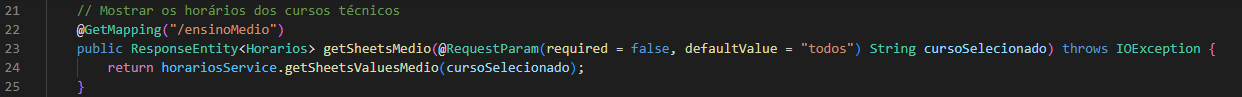
\includegraphics[width=1\textwidth]{Figuras/back-3.png}
        \caption*{Fonte: AUTOR (2025)}
        \label{fig_back_3}
    \end{figure}

    O objetivo do endpoint apresentado na Figura \ref{fig_back_3} é retornar os horários dos cursos técnicos. O parâmetro utilizado é cursoSelecionado, que é opcional e, por padrão, assume o valor "todos". Tendo isso como referência, o sistema consulta os dados na planilha e os retorna de forma organizada dentro de um objeto Horarios com os horários de todos os cursos técnicos ou de um curso técnico específico.

    \begin{figure}[htb]
        \centering
        \caption{Endpoint de consulta dos horários dos cursos superiores}
        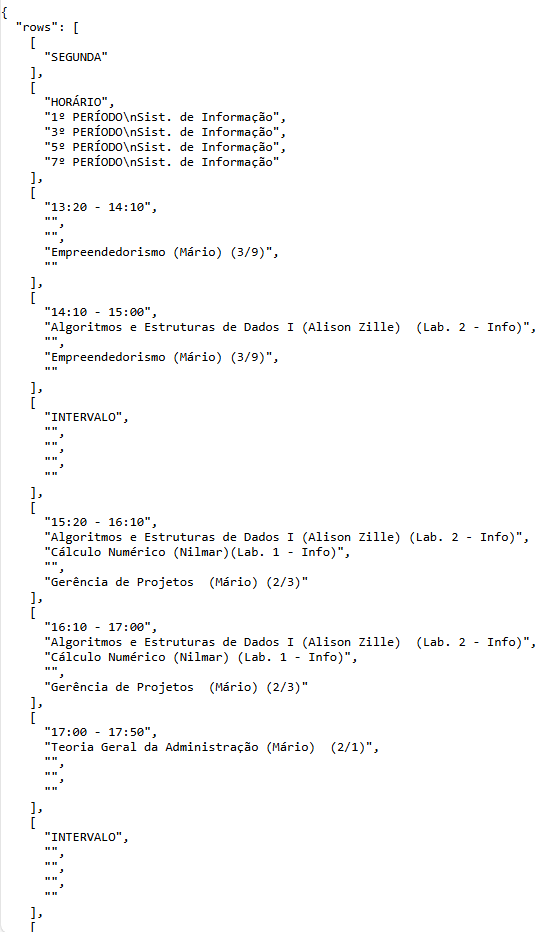
\includegraphics[width=1\textwidth]{Figuras/back-4.png}
        \caption*{Fonte: AUTOR (2025)}
        \label{fig_back_4}
    \end{figure}

    O objetivo do endpoint apresentado na Figura \ref{fig_back_4} é retornar os horários dos cursos superiores. O parâmetro utilizado é cursoSelecionado, que é opcional e, por padrão, assume o valor "todos". Tendo isso como referência, o sistema consulta os dados na planilha e os retorna de forma organizada dentro de um objeto Horarios com os horários de todos os cursos superiores ou de um curso superior específico.

    \begin{figure}[htb]
        \centering
        \caption{Endpoint de consulta dos horários dos professores}
        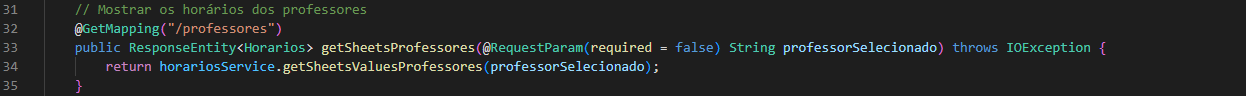
\includegraphics[width=1\textwidth]{Figuras/back-5.png}
        \caption*{Fonte: AUTOR (2025)}
        \label{fig_back_5}
    \end{figure}

    Conforme ilustrado na Figura \ref{fig_back_5}, o objetivo do endpoint é retornar os horários dos professores. O parâmetro professorSelecionado é opcional e pode ser deixado em branco. Com base nisso, o sistema consulta os dados na planilha e os retorna de forma organizada dentro de um objeto Horarios com os horários de um professor específico.

    \begin{figure}[htb]
        \centering
        \caption{Endpoint de consulta dos horários de ocupação das salas}
        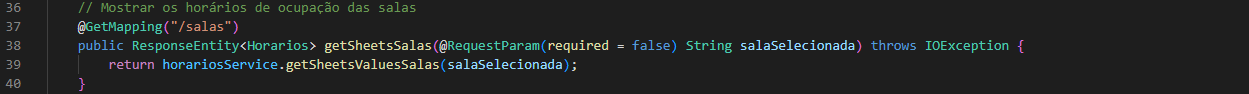
\includegraphics[width=1\textwidth]{Figuras/back-6.png}
        \caption*{Fonte: AUTOR (2025)}
        \label{fig_back_6}
    \end{figure}

    Conforme ilustrado na Figura \ref{fig_back_6}, o objetivo do endpoint é retornar os horários de ocupação das salas. O parâmetro salaSelecionada é opcional e pode ser deixado em branco. Com base nisso, o sistema consulta os dados na planilha e os retorna de forma organizada dentro de um objeto Horarios com os horários de ocupação de uma sala específica.

    \begin{figure}[htb]
        \centering
        \caption{Endpoint de consulta das permissões para ver validação da planiha}
        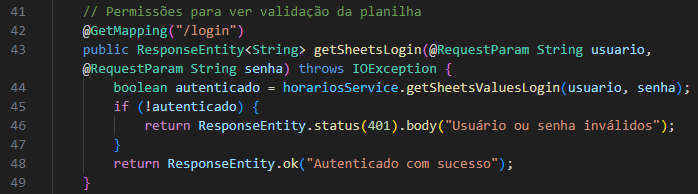
\includegraphics[width=1\textwidth]{Figuras/back-7.png}
        \caption*{Fonte: AUTOR (2025)}
        \label{fig_back_7}
    \end{figure}

    Como mostrado na Figura \ref{fig_back_7}, o objetivo do endpoint é validar as credenciais de acesso informadas. Os parâmetros obrigatórios são usuario e senha. Com essas informações, o sistema realiza a autenticação e retorna uma mensagem com o status correspondente, sendo 200 em caso de sucesso ou 401 não autorizado caso as credenciais estejam incorretas.

    \begin{figure}[H]
        \centering
        \caption{Endpoint de consulta para validar dados da planilha}
        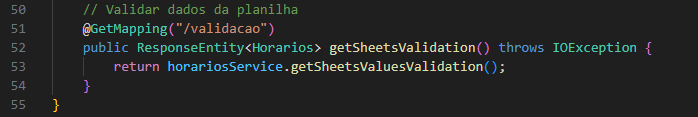
\includegraphics[width=1\textwidth]{Figuras/back-8.png}
        \caption*{Fonte: AUTOR (2025)}
        \label{fig_back_8}
    \end{figure}

    Conforme mostrado na Figura \ref{fig_back_8}, o objetivo do endpoint é retornar os resultados da validação dos dados da planilha de horários. Nenhum parâmetro é necessário para a execução da requisição. Ao ser acionado, o sistema analisa a planilha e responde com um objeto Horarios contendo eventuais inconsistências ou erros detectados durante o processo de validação.
\end{itemize}

\section{Deploy}

O front-end foi hospedado na plataforma Vercel, permitindo a disponibilização da interface do usuário com alta performance e integração contínua, como mostrado na Figura \ref{fig_deploy_1}.

\begin{figure}[htb]
    \centering
    \caption{Deploy do front-end da plataforma na Vercel}
    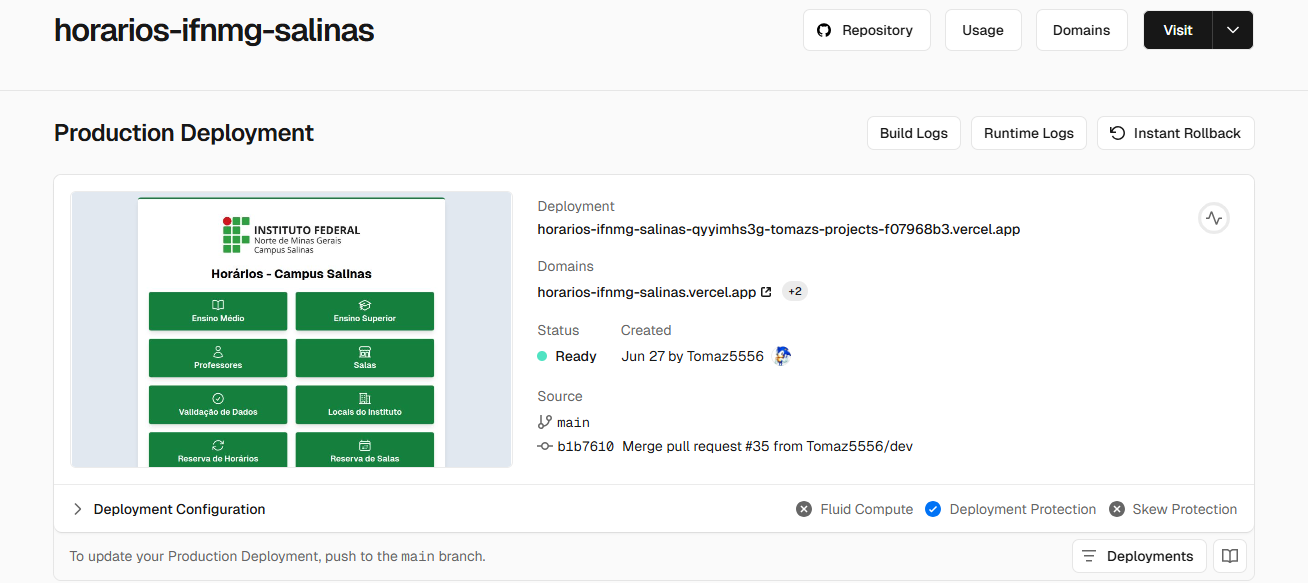
\includegraphics[width=1\textwidth]{Figuras/deploy-1.png}
    \caption*{Fonte: AUTOR (2025)}
    \label{fig_deploy_1}
\end{figure}

Já o back-end foi hospedado na plataforma Koyeb, responsável por executar a API que processa e envia os dados do Google Sheets ao front-end, conforme ilustrado na Figura \ref{fig_deploy_2}.

\begin{figure}[H]
    \centering
    \caption{Deploy do back-end da plataforma na Koyeb}
    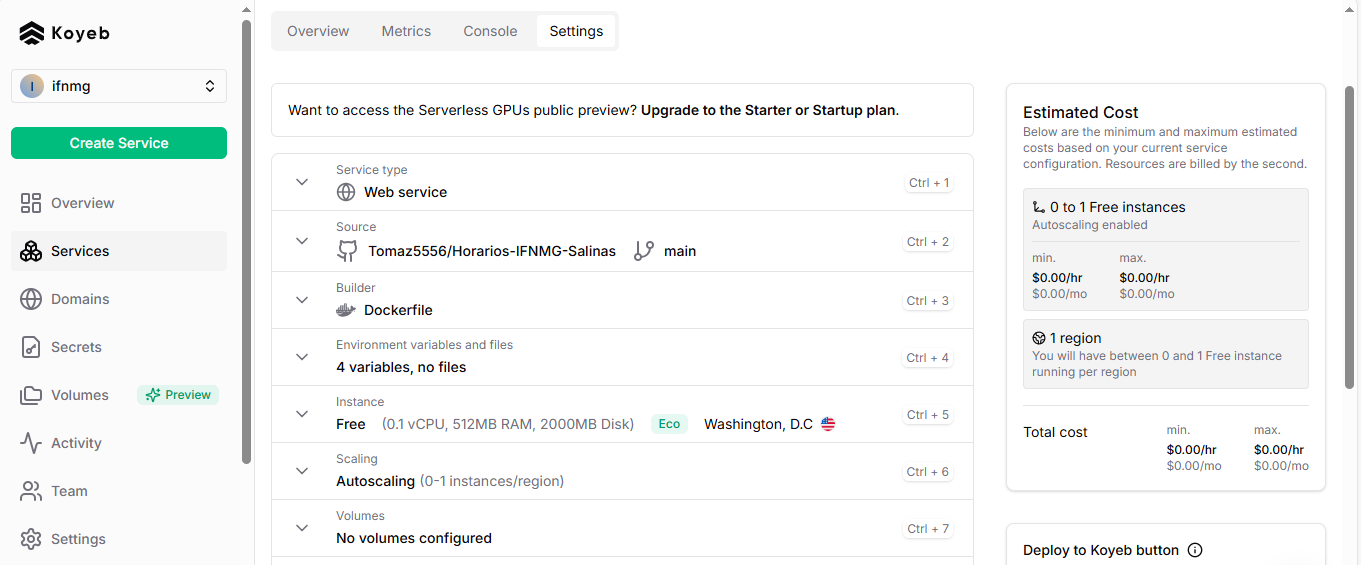
\includegraphics[width=1\textwidth]{Figuras/deploy-2.png}
    \caption*{Fonte: AUTOR (2025)}
    \label{fig_deploy_2}
\end{figure}

\section{Documentação}

As Figuras \ref{fig_doc_1}, \ref{fig_doc_2} e \ref{fig_doc_3} apresentam a documentação técnica elaborada para a planilha utilizada como banco de dados do sistema. A documentação está disponível no seguinte endereço \url{https://tomaz5556.github.io/Horarios-IFNMG-Salinas}. Esse material descreve, de forma clara e objetiva, as instruções para atualização do identificador da planilha, as regras de preenchimento dos dados, bem como os padrões de nomes e intervalos de células necessários para garantir a integridade do funcionamento da plataforma.

\begin{figure}[htb]
    \centering
    \caption{Instruções para desenvolvedores}
    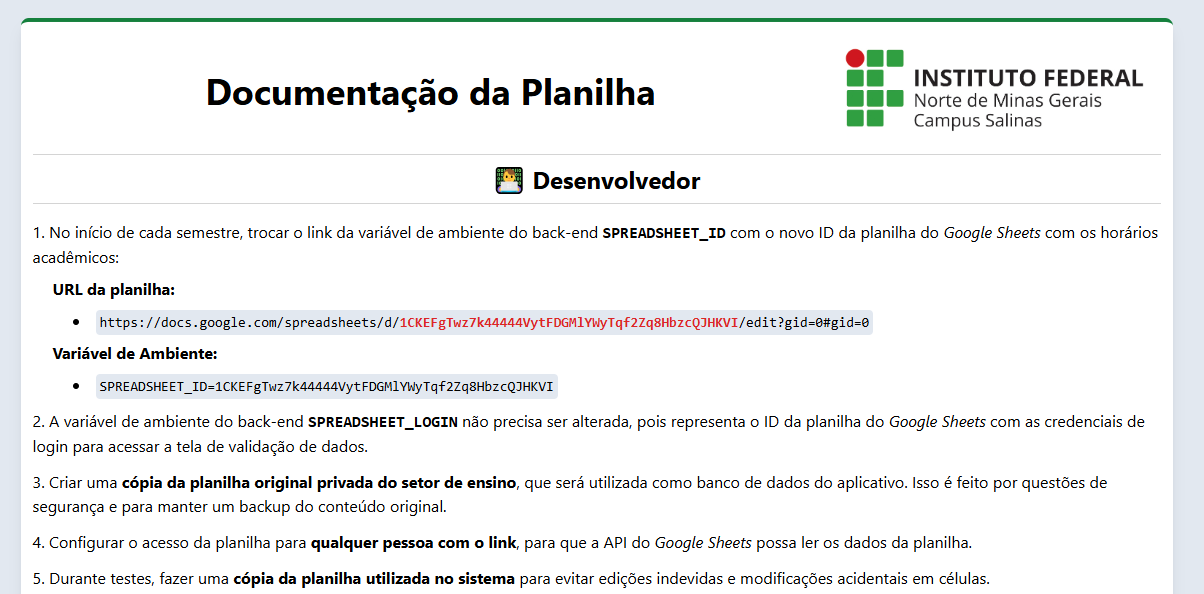
\includegraphics[width=0.9\textwidth]{Figuras/doc-1.png}
    \caption*{Fonte: AUTOR (2025)}
    \label{fig_doc_1}
\end{figure}

\begin{figure}[htb]
    \centering
    \caption{Instruções para administradores da planilha}
    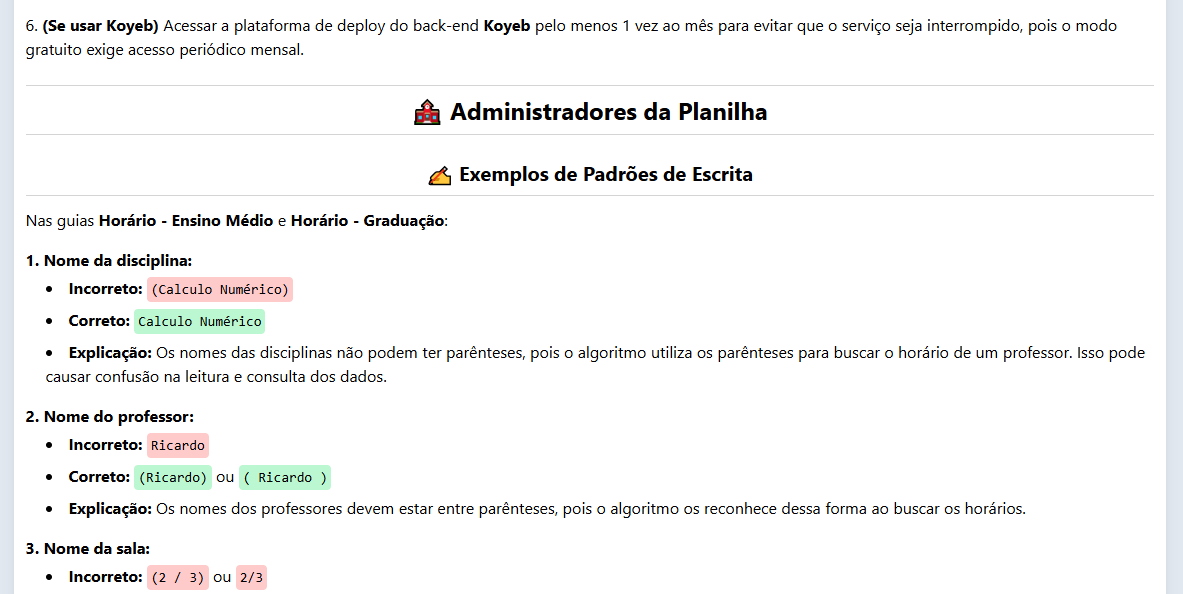
\includegraphics[width=0.9\textwidth]{Figuras/doc-2.png}
    \caption*{Fonte: AUTOR (2025)}
    \label{fig_doc_2}
\end{figure}

\begin{figure}[htb]
    \centering
    \caption{Explicação das guias e intervalos de células}
    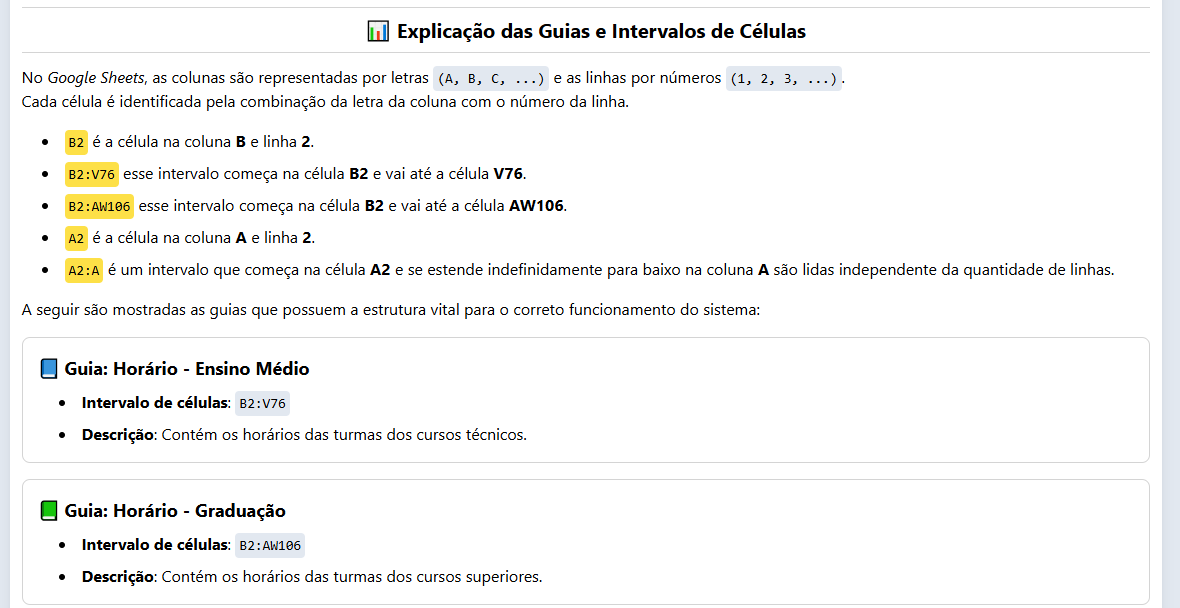
\includegraphics[width=0.9\textwidth]{Figuras/doc-3.png}
    \caption*{Fonte: AUTOR (2025)}
    \label{fig_doc_3}
\end{figure}

\begin{figure}[htb]
    \centering
    \caption{Observação sobre mudanças estruturais}
    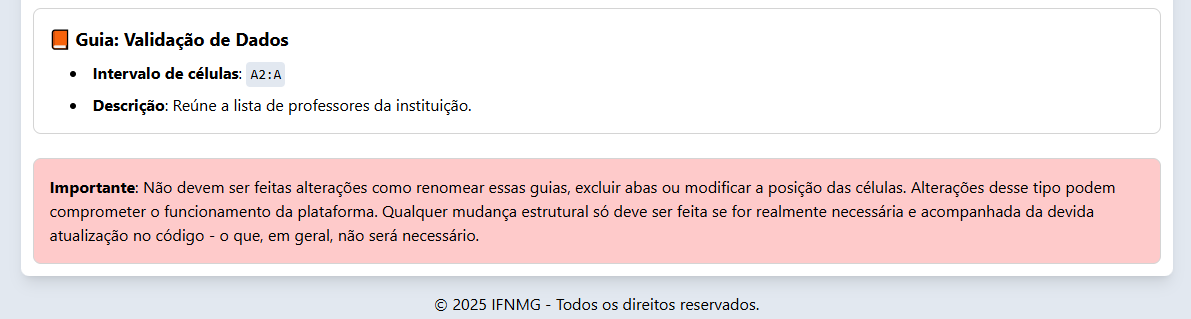
\includegraphics[width=0.9\textwidth]{Figuras/doc-4.png}
    \caption*{Fonte: AUTOR (2025)}
    \label{fig_doc_4}
\end{figure}